\chapter{APP AS A DATA ANALYSIS TOOL}
\label{chap:analysis_tool}

\textbf{Data analysis} is a tool used to examine, clean, change and rebuild information with a view to reach to a specific decision for a given circumstance. Information investigation is normally of two sorts: subjective or quantitative. During the research procedure any non-numerical information like content or individual words are broke down. Quantitative examination, then again, centers around estimation of the information and can utilize insights to help uncover results. The outcomes are numerical. At times, the two types of examination are utilized as an inseparable unit. For instance, quantitative investigation can help demonstrate subjective ends. Spatial information investigation is concerned about that part of information examination where the land referencing of articles contains imperative data. This chapter talks about the ways this app can be used as an analysis tool directly or indirectly. \\

\section{Data downloading}

\textbf{Downloading} is defined as the transfer of data from the server to the system. This is defined as the transmission of data from one machine to another. The significant advantage of downloading is that it gives the user the full access over the downloaded data with the goal to utilize the information. The app gives users the feature of exporting any admim level (0, 1 or 2) data in \gls{csv} format via email so that it can be used in any form of spatial analysis. Tghe process of data downloading is described below.

\begin{itemize}
    \item Select the date and tap on country to see the data and then tap on any region. Once that is done, users can see two buttons on both top corners of the screen. Figure~\ref{fig:buttons} shows the two buttons which appears after having valid data on globe / map. \\
    
      \begin{figure}[H]
            \centering
            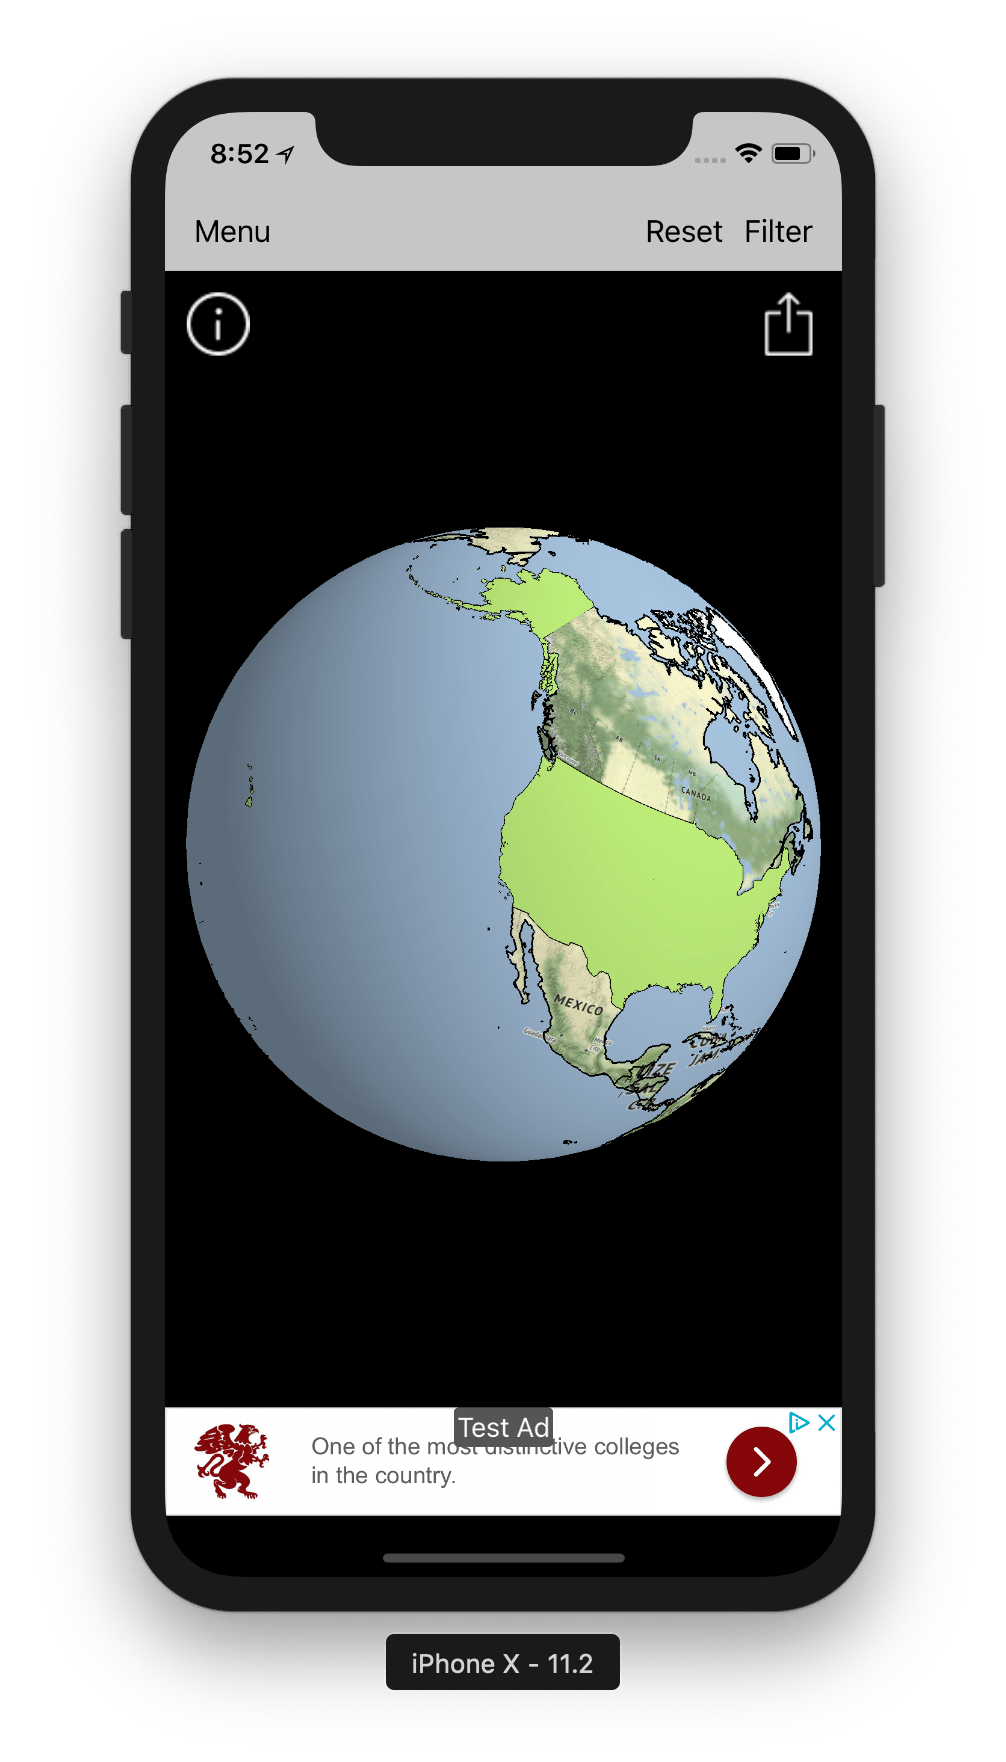
\includegraphics[width=0.25\linewidth]{figures/ch5/buttons.png}
            \caption{\label{fig:buttons} Home screen with two buttons on top corners}
        \end{figure}
     
    \item Left button in Figure~\ref{fig:buttons} corresponds to Information button which shows information about the current data being displayed. Figure~\ref{fig:info_button} shows the view appears on tapping the information button. \\
    
      \begin{figure}[H]
            \centering
            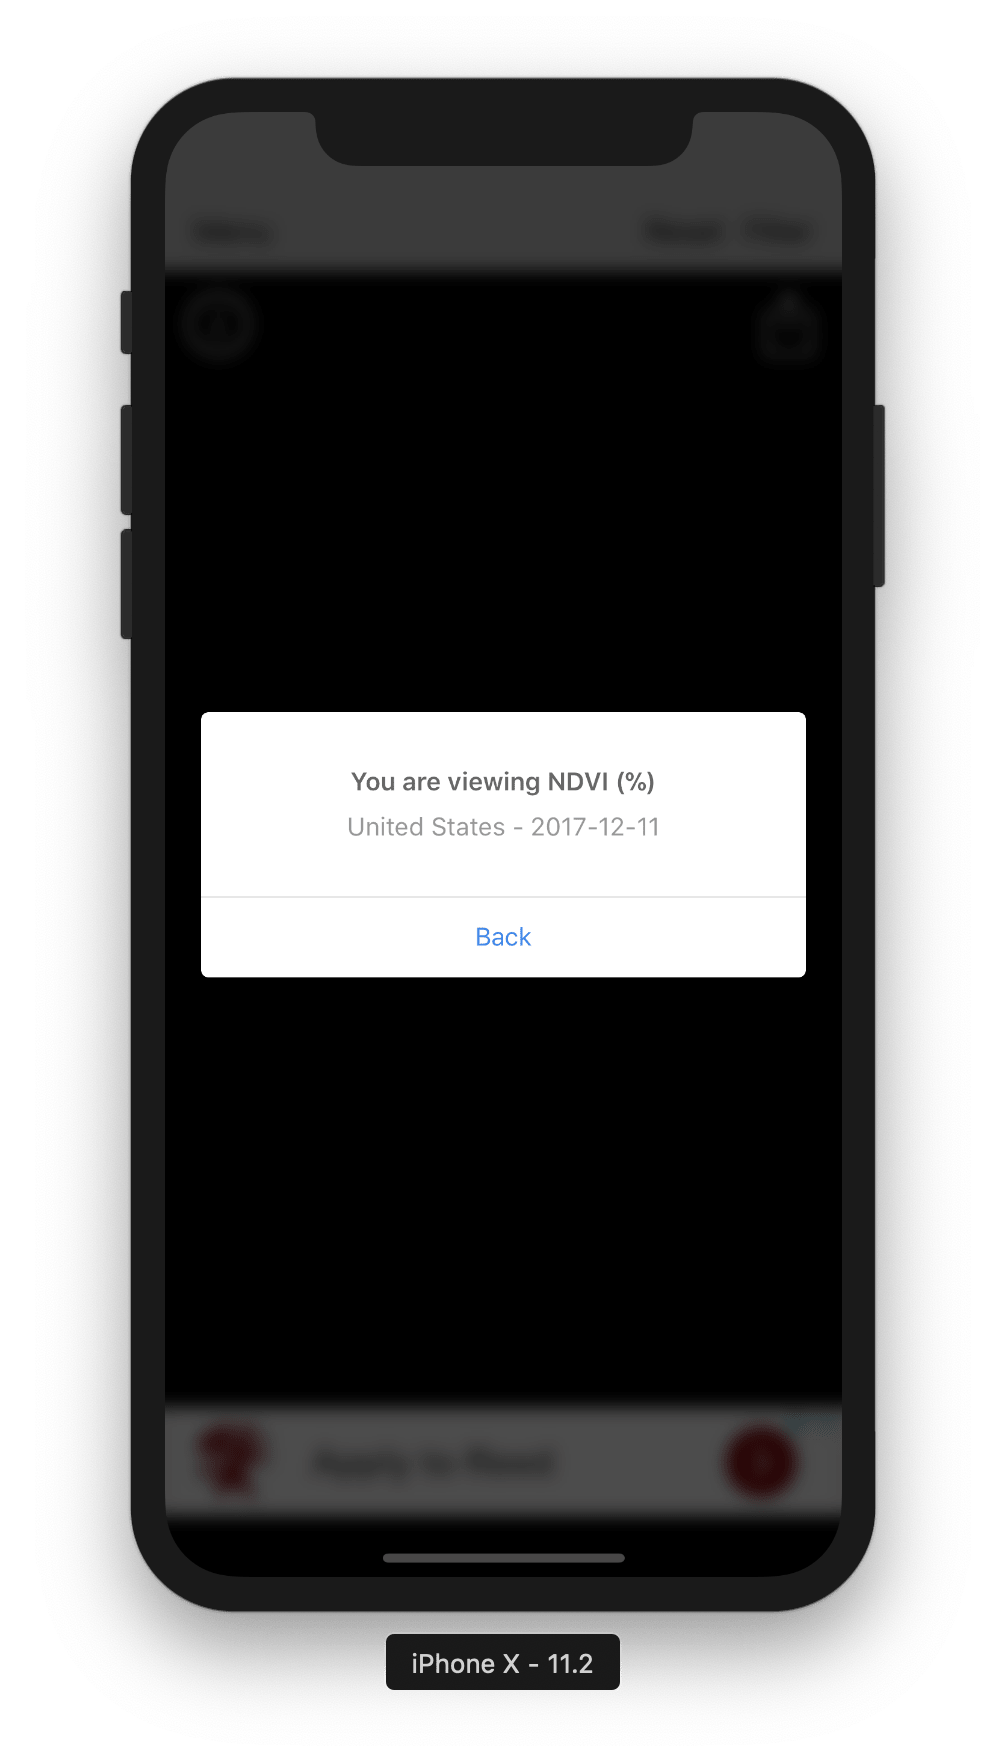
\includegraphics[width=0.25\linewidth]{figures/ch5/info_view.png}
            \caption{\label{fig:info_button} Information button action}
        \end{figure}
       
     \item Right button in Figure~\ref{fig:buttons} corresponds to export button which prompts users to export the current data in \gls{csv} format via email which is visible on globe / map. Figure~\ref{fig:export_button} shows the export view by tapping of export button. \\
     
     \begin{figure}[H]
            \centering
            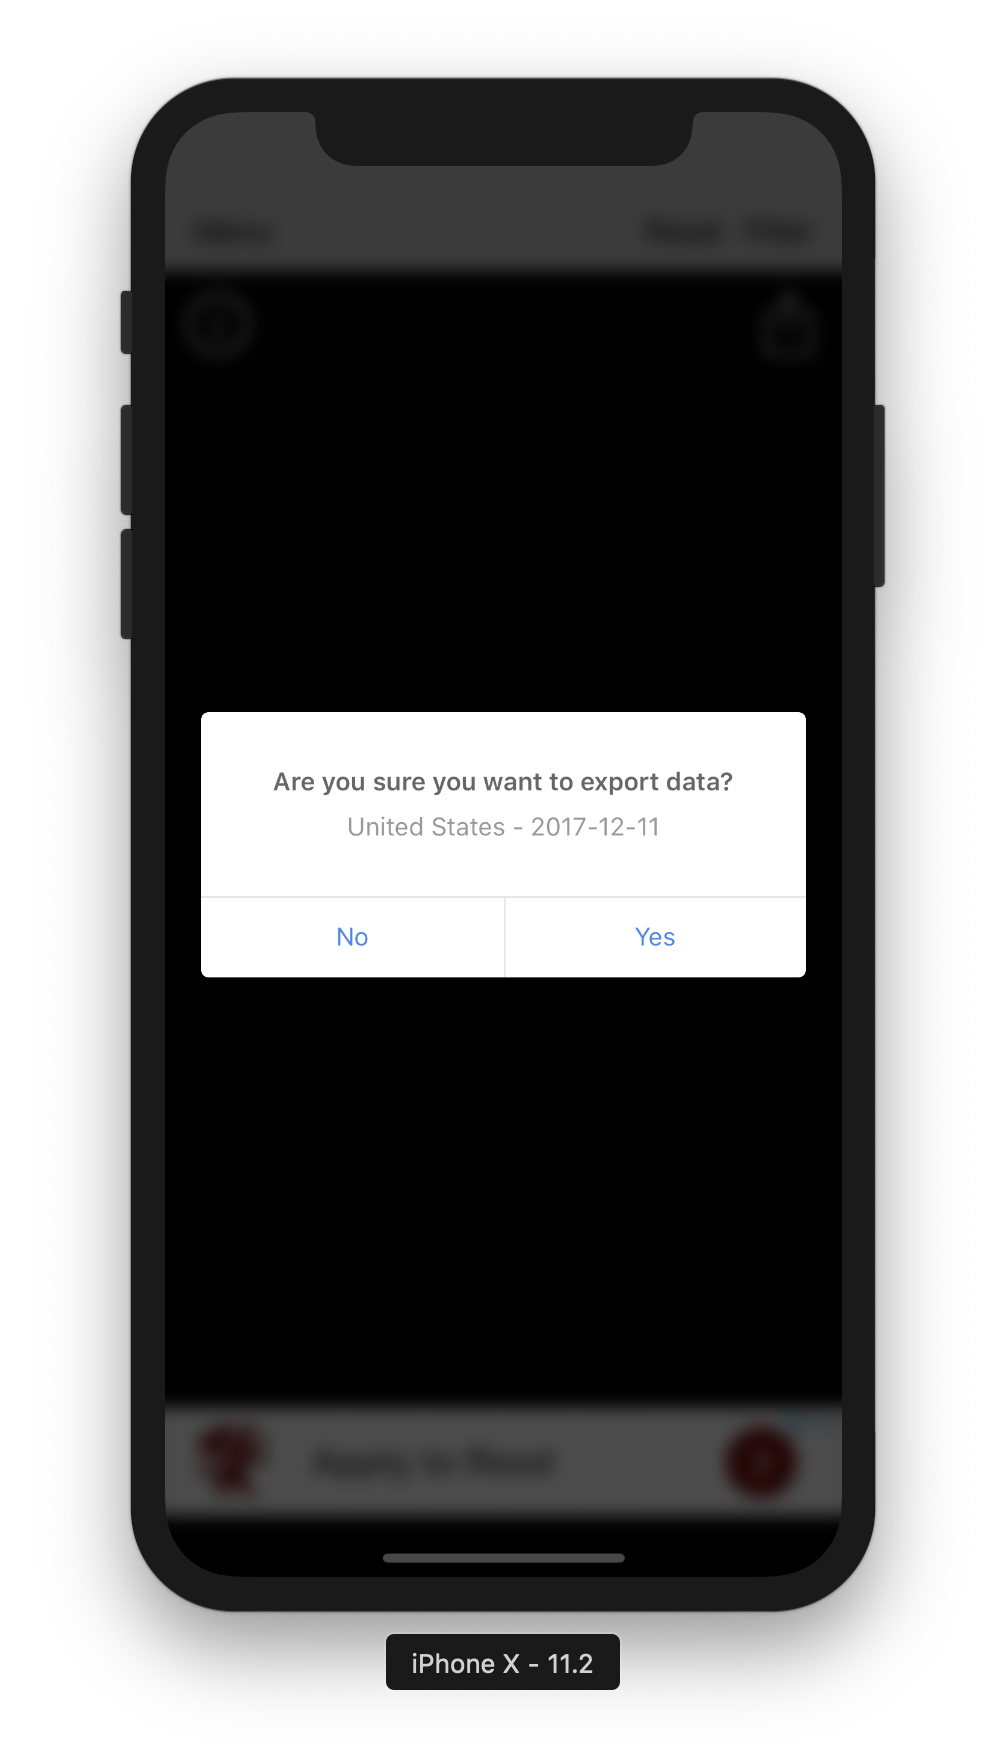
\includegraphics[width=0.25\linewidth]{figures/ch5/export_view.png}
            \caption{\label{fig:export_button} Export button action on home screen}
    \end{figure}
    
    By selecting yes in Figure~\ref{fig:export_button}, \gls{json} data is converted to a valid \gls{csv} format and attached as a file on the MFMailComposeViewController. According to Apple, this is a standard interface for managing, editing, and sending email messages in \gls{iOS} app\cite{MFMailComposer}. Figure~\ref{fig:email_controller} shows the MFMailComposerViewController view which helps user to email the \gls{csv} file. 
    
    \begin{figure}[H]
            \centering
            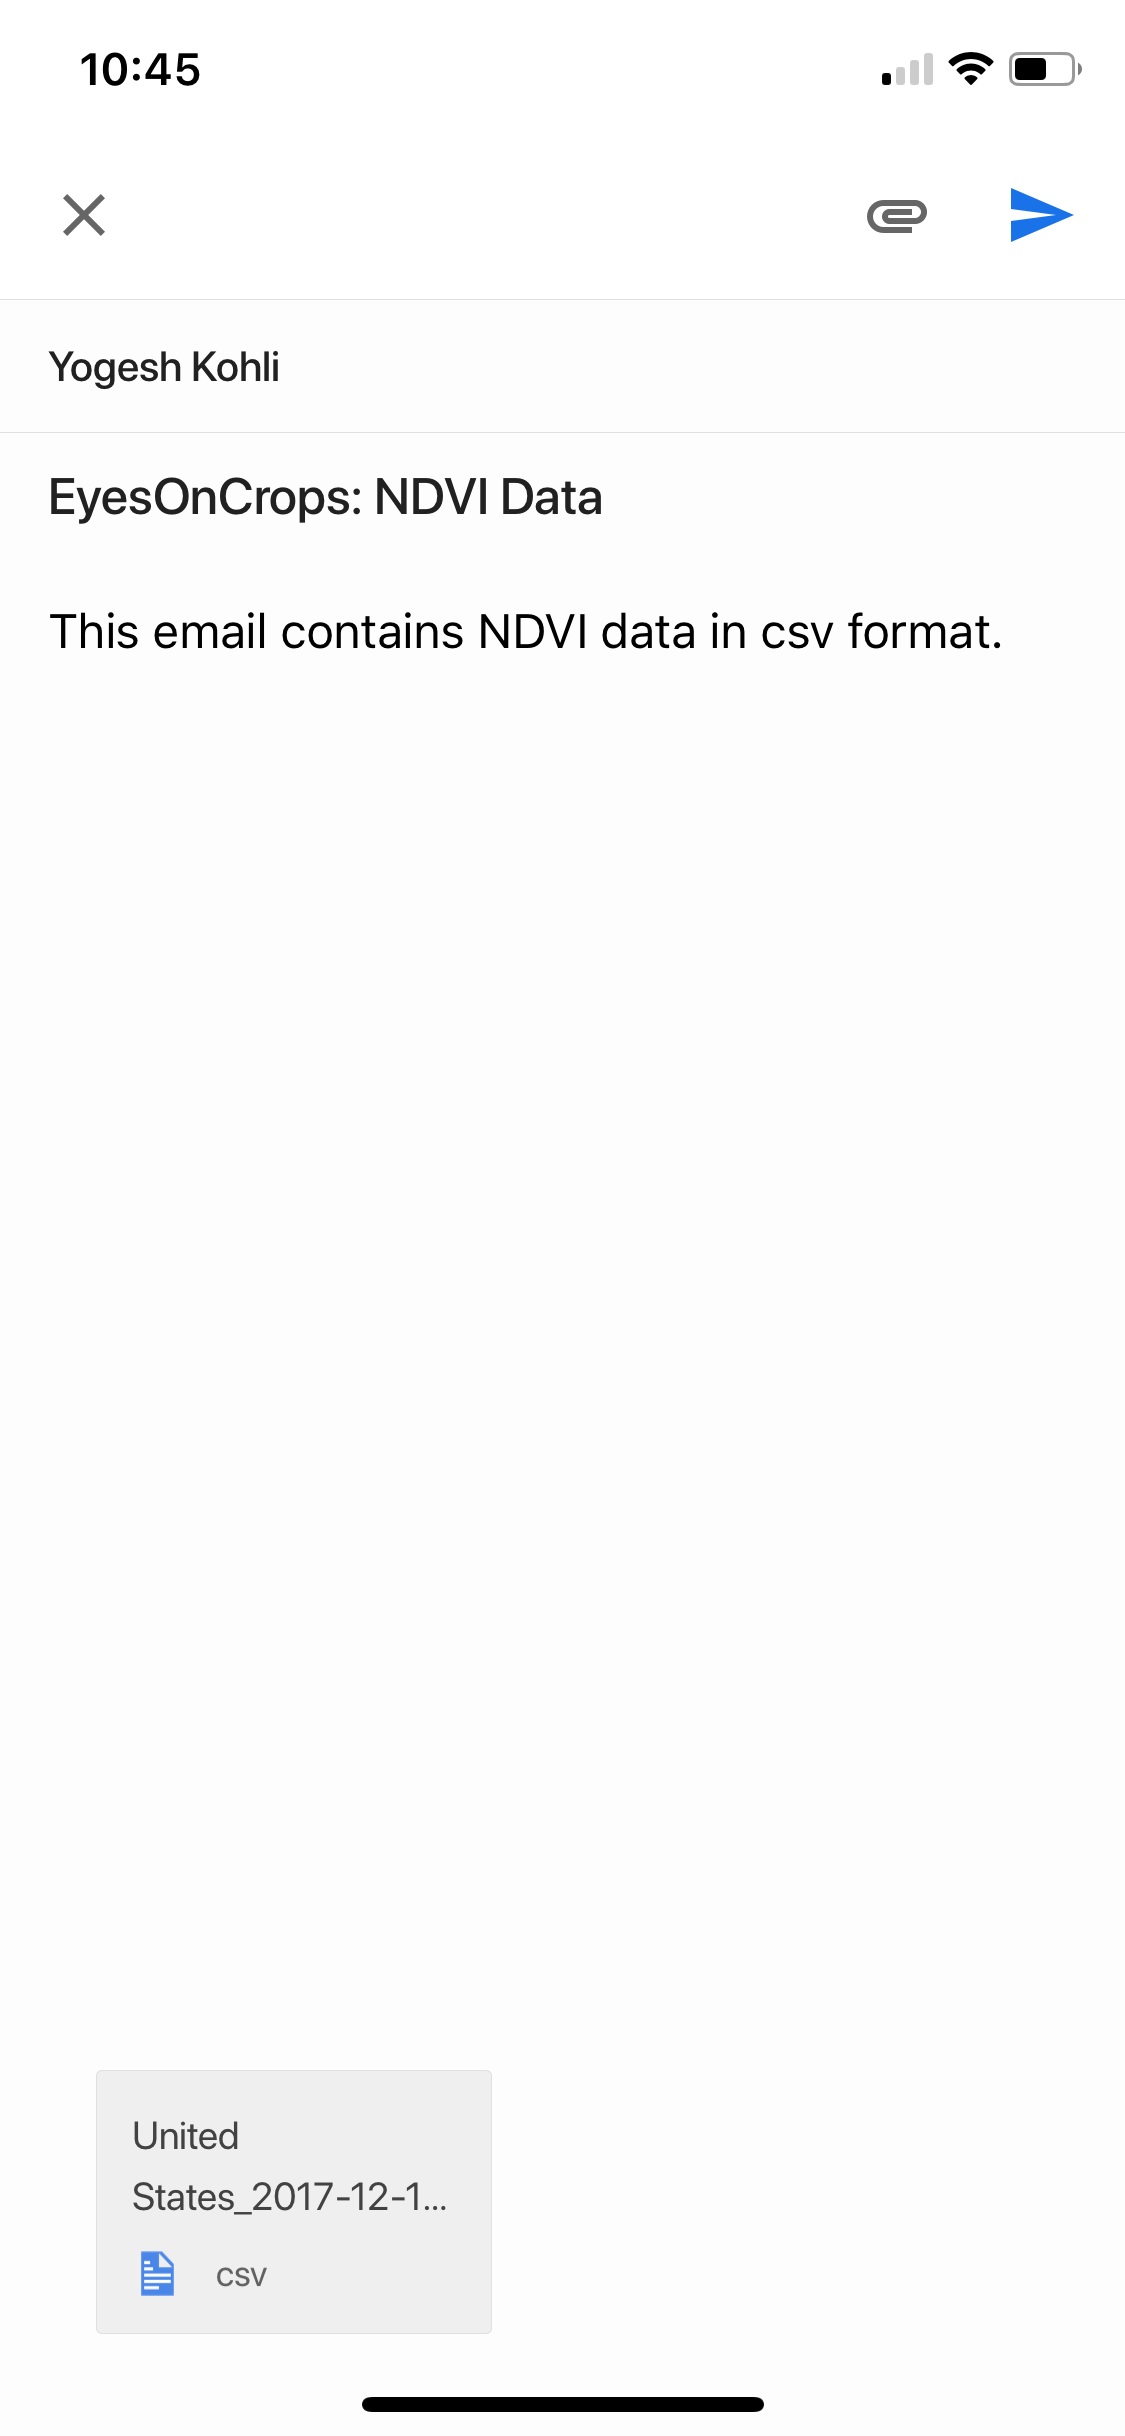
\includegraphics[width=0.25\linewidth]{figures/ch5/mfmailcomposer.png}
            \caption{\label{fig:email_controller} Email controller after selecting yes on export action screen}
    \end{figure}
    
\end{itemize}


\section{Computing mean, standard deviation and histogram}

\begin{itemize}
    \item \textbf{Mean} \\
    According to a paper published about Descriptive Statistics in 1997, the mean of a data is simply the arithmetic average of the values in the set, attained by summing the values and dividing by the number of values. Remember, when summarizing a data set in a frequency distribution, the data is being approximated (rounded). With this in mind, it is natural to define the mean of a frequency distribution by Figure 5.5 \cite{Mean_SD}.
    
    \begin{equation} \label{eq:mean_formula}
       \mu = \frac{1}{n} \sum\limits_{i=1}^{n}f_{i}x_{i} \doteq \sum\limits_{i=1}^{n}p_{i}x_{i}
    \end{equation}
    
    \item \textbf{Standard Deviation} \\
   It is defined as the amount computed to show the degree of deviation for a gathering all in all. Where $\sigma$ represents the standard deviation, $x_{i}$ are the individual values and $\mu$ represents the mean which can be calculated by Equation 5.1.
   
  \begin{equation} \label{eq:standarddeviation_formula}
      \sigma = \sqrt{\frac{\sum\limits_{i=1}^{n}(x_{i} - \mu)^2}{n}}
    \end{equation}
    


    
\end{itemize}

\centerline{\textbf{Why use mean and standard deviation for analysis?}}

The main purpose of using mean and standard deviation as a parameter for analysis is that the Normal Curve discloses pattern around a normal line whereas Standard deviation is viewed as the most valuable list of variability. It discloses to us the inconstancy, or spread, of an appropriation (gathering of scores). This paper investigates \gls{ndvi} and Anomaly data for some regions to demonstrate with the information through the app. The user is able to do the following:

\begin{itemize}
    \item \textbf{Mean NDVI \& Anomaly distribution over the years}
    
     \begin{figure}[H]
            \centering
            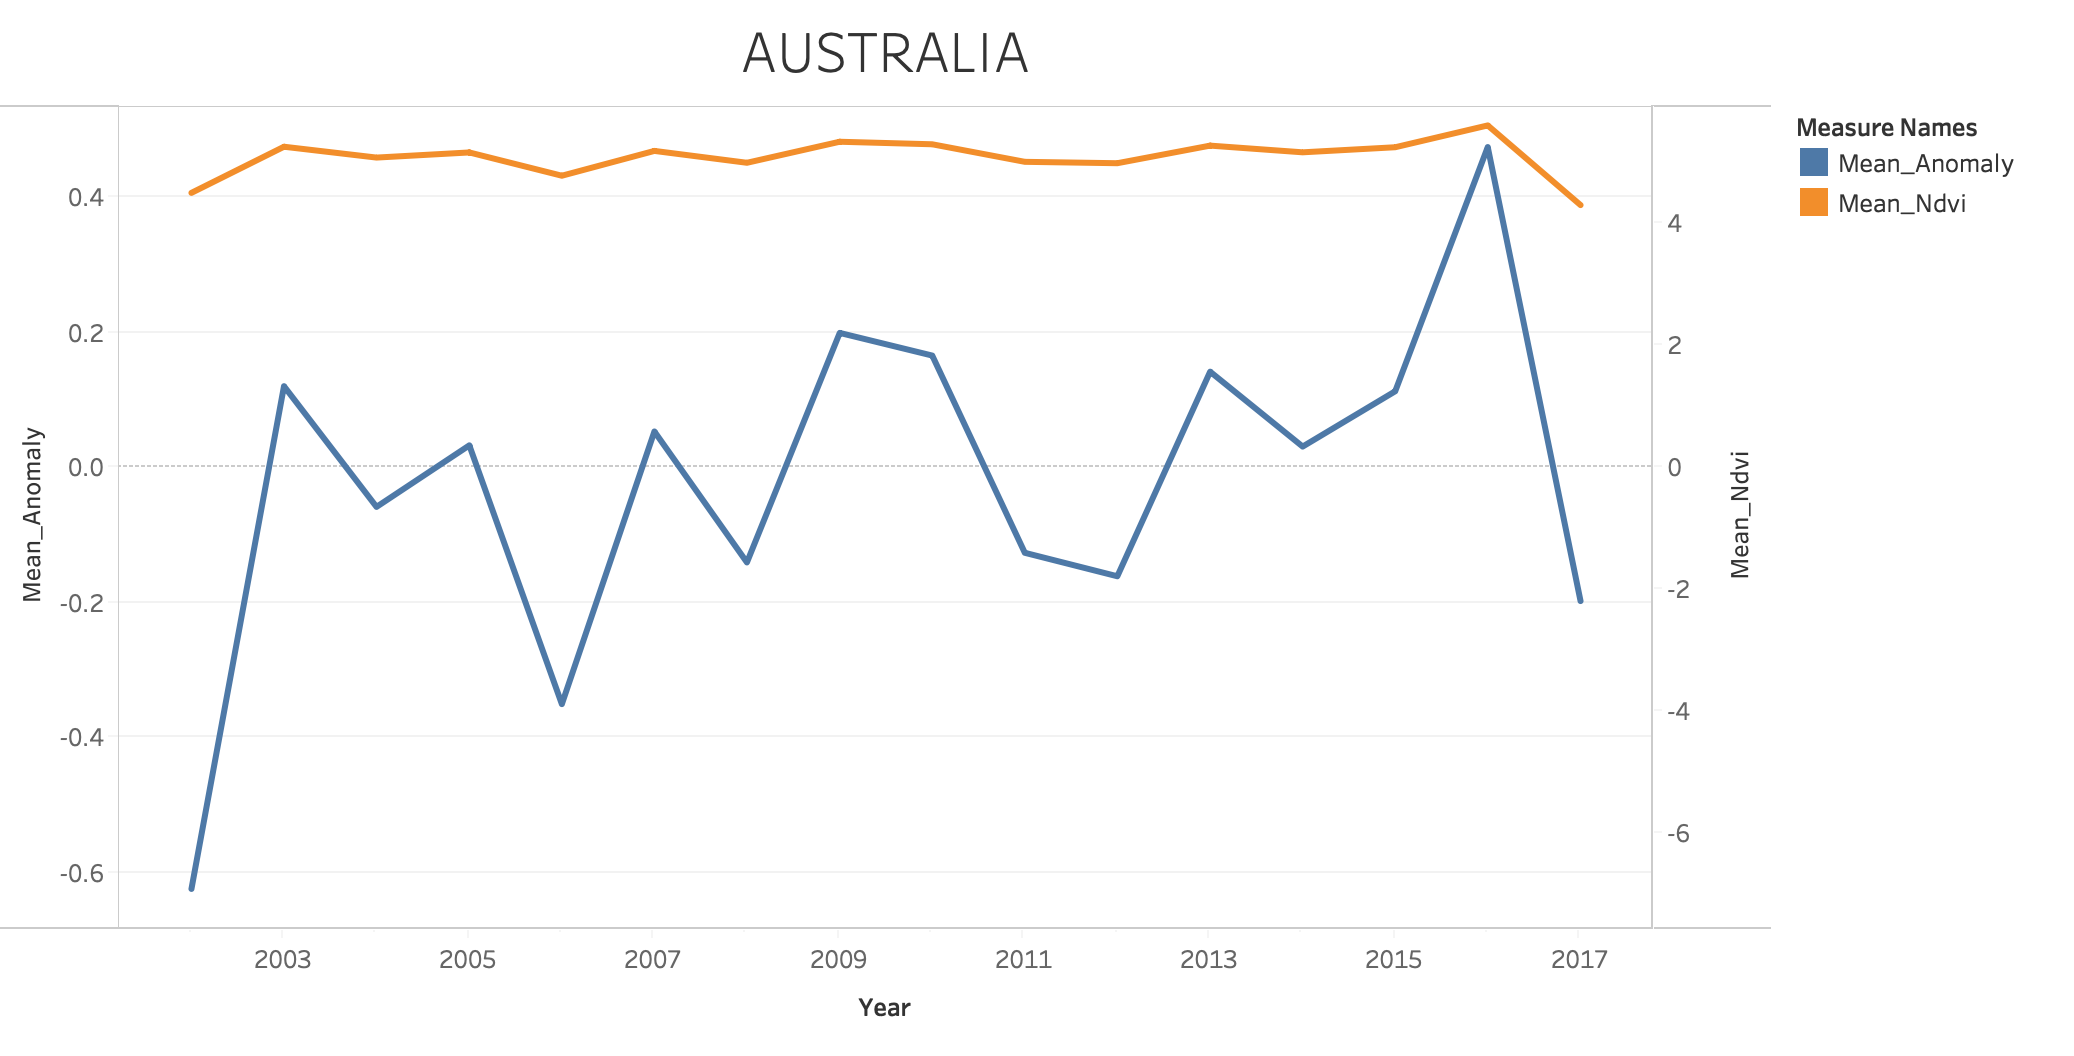
\includegraphics[width=1.0\linewidth]{figures/ch5/Mean/AUSTRALIA_mean.png}
            \caption{Mean graph - Australia}\label{Fig:AUSTRALIA_mean}
    \end{figure}
    
    \begin{figure}[H]
            \centering
            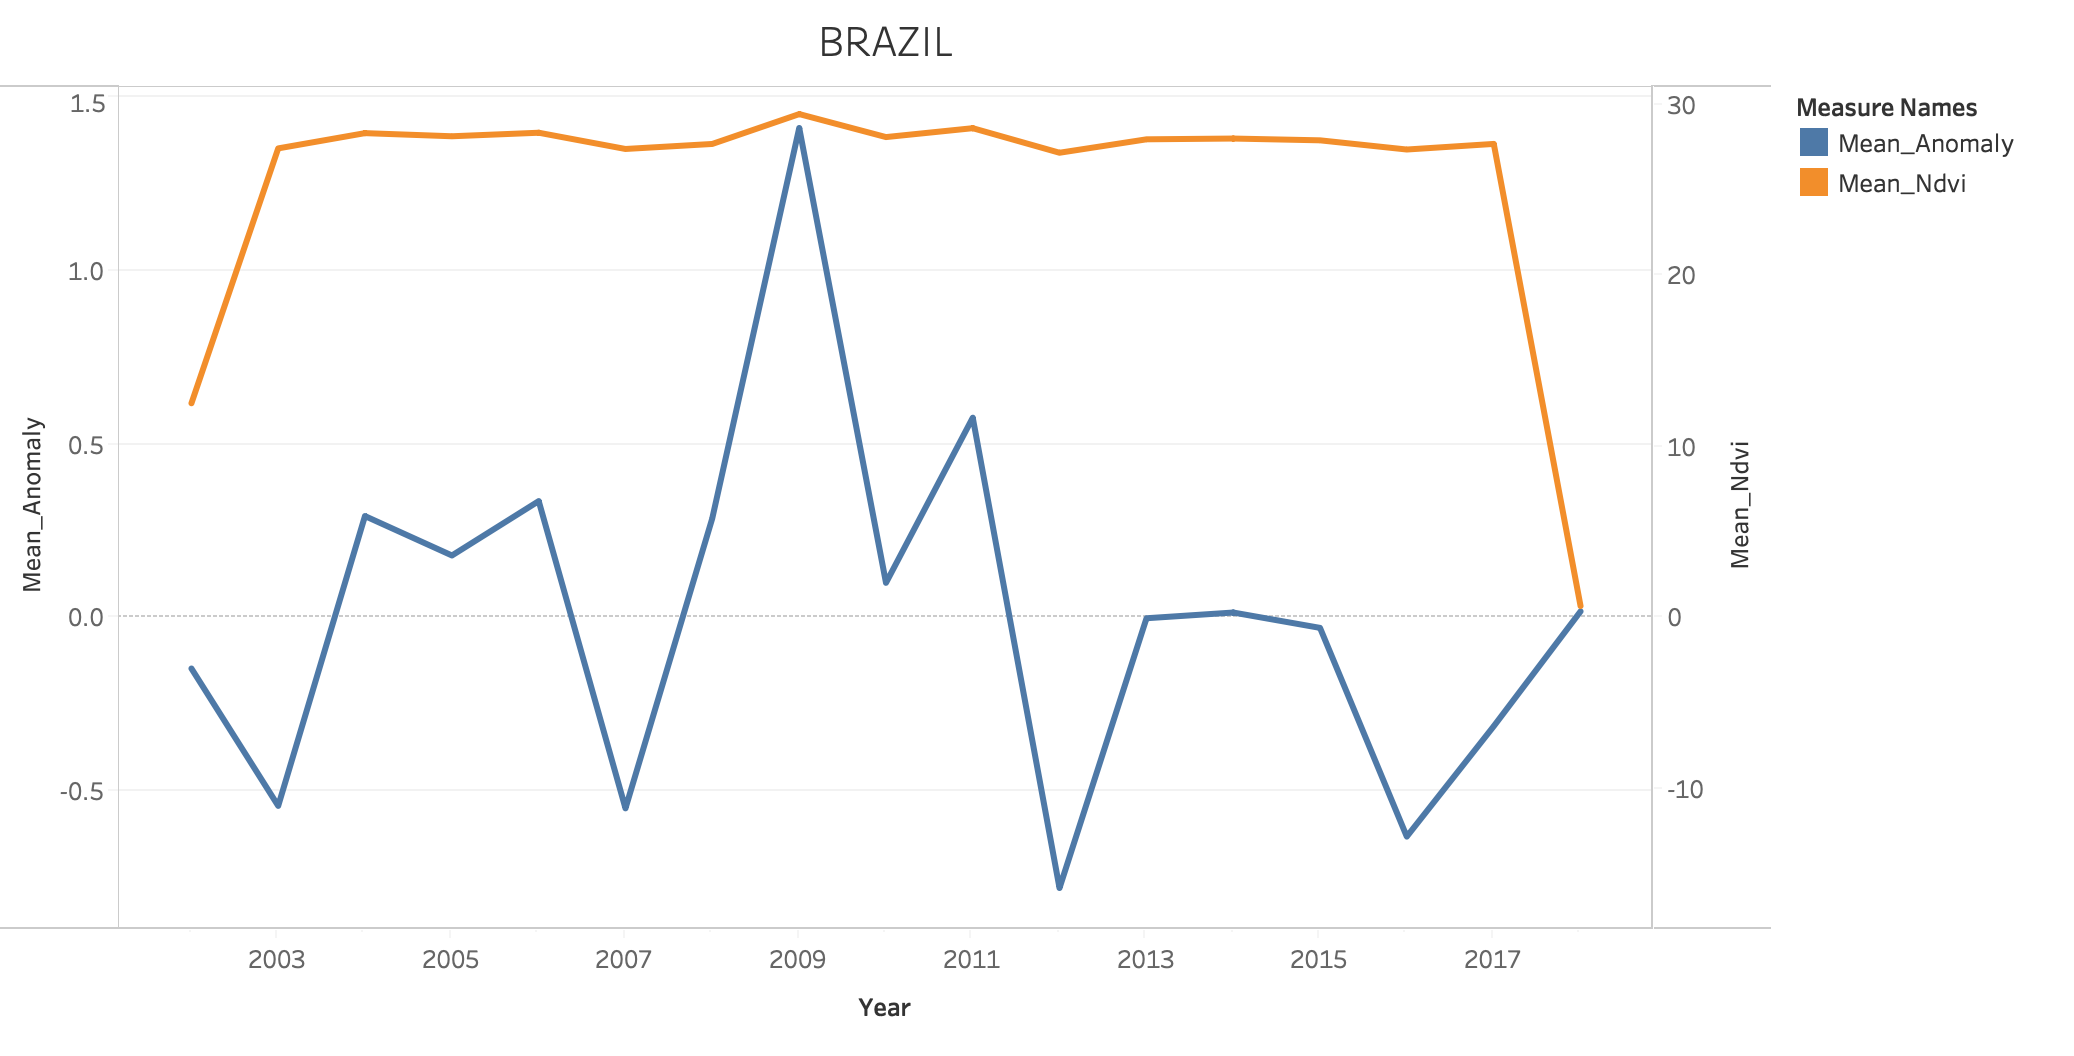
\includegraphics[width=1.0\linewidth]{figures/ch5/Mean/BRAZIL_mean.png}
            \caption{Mean graph - Brazil}\label{Fig:BRAZIL_mean}
    \end{figure}
    
    \begin{figure}[H]
            \centering
            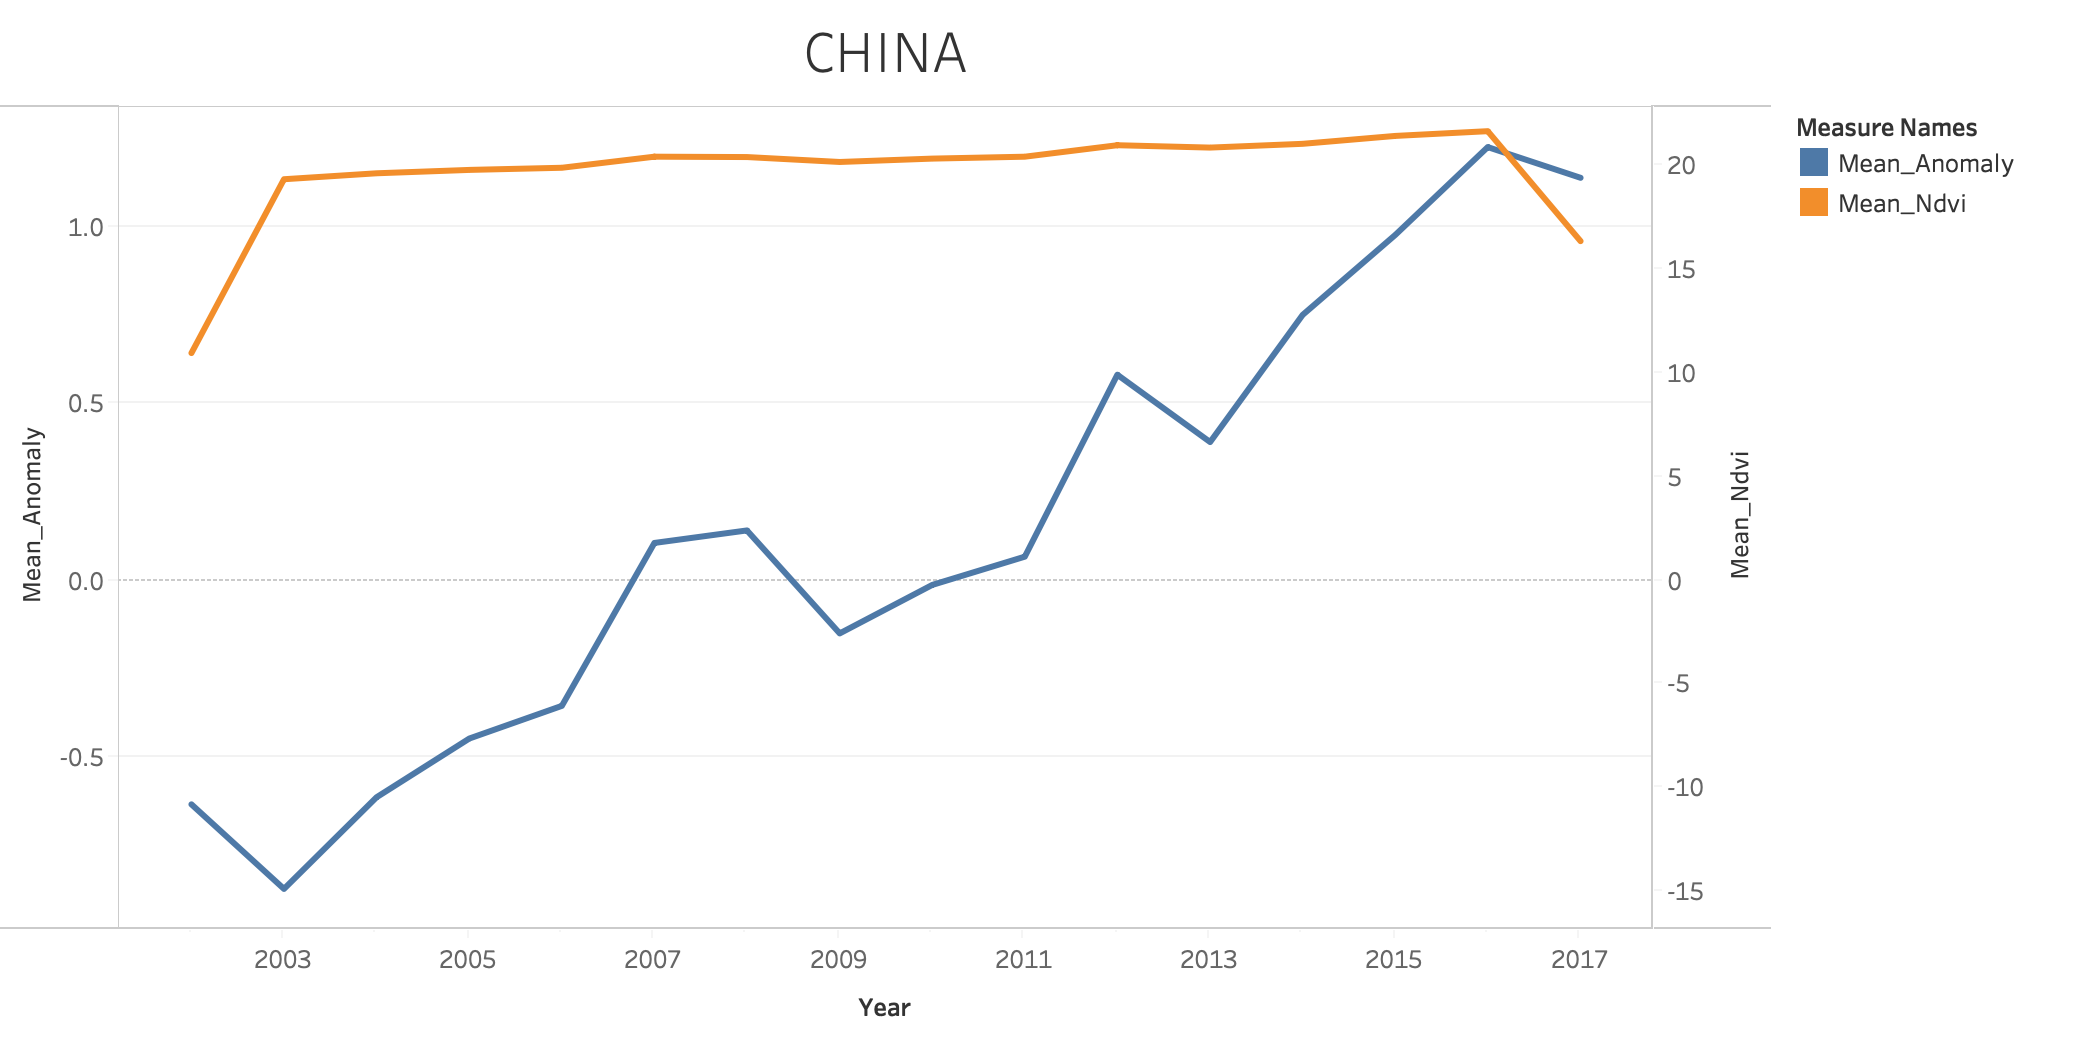
\includegraphics[width=1.0\linewidth]{figures/ch5/Mean/CHINA_mean.png}
            \caption{Mean graph - China}\label{Fig:CHINA_mean}
    \end{figure}
    
    \begin{figure}[H]
            \centering
            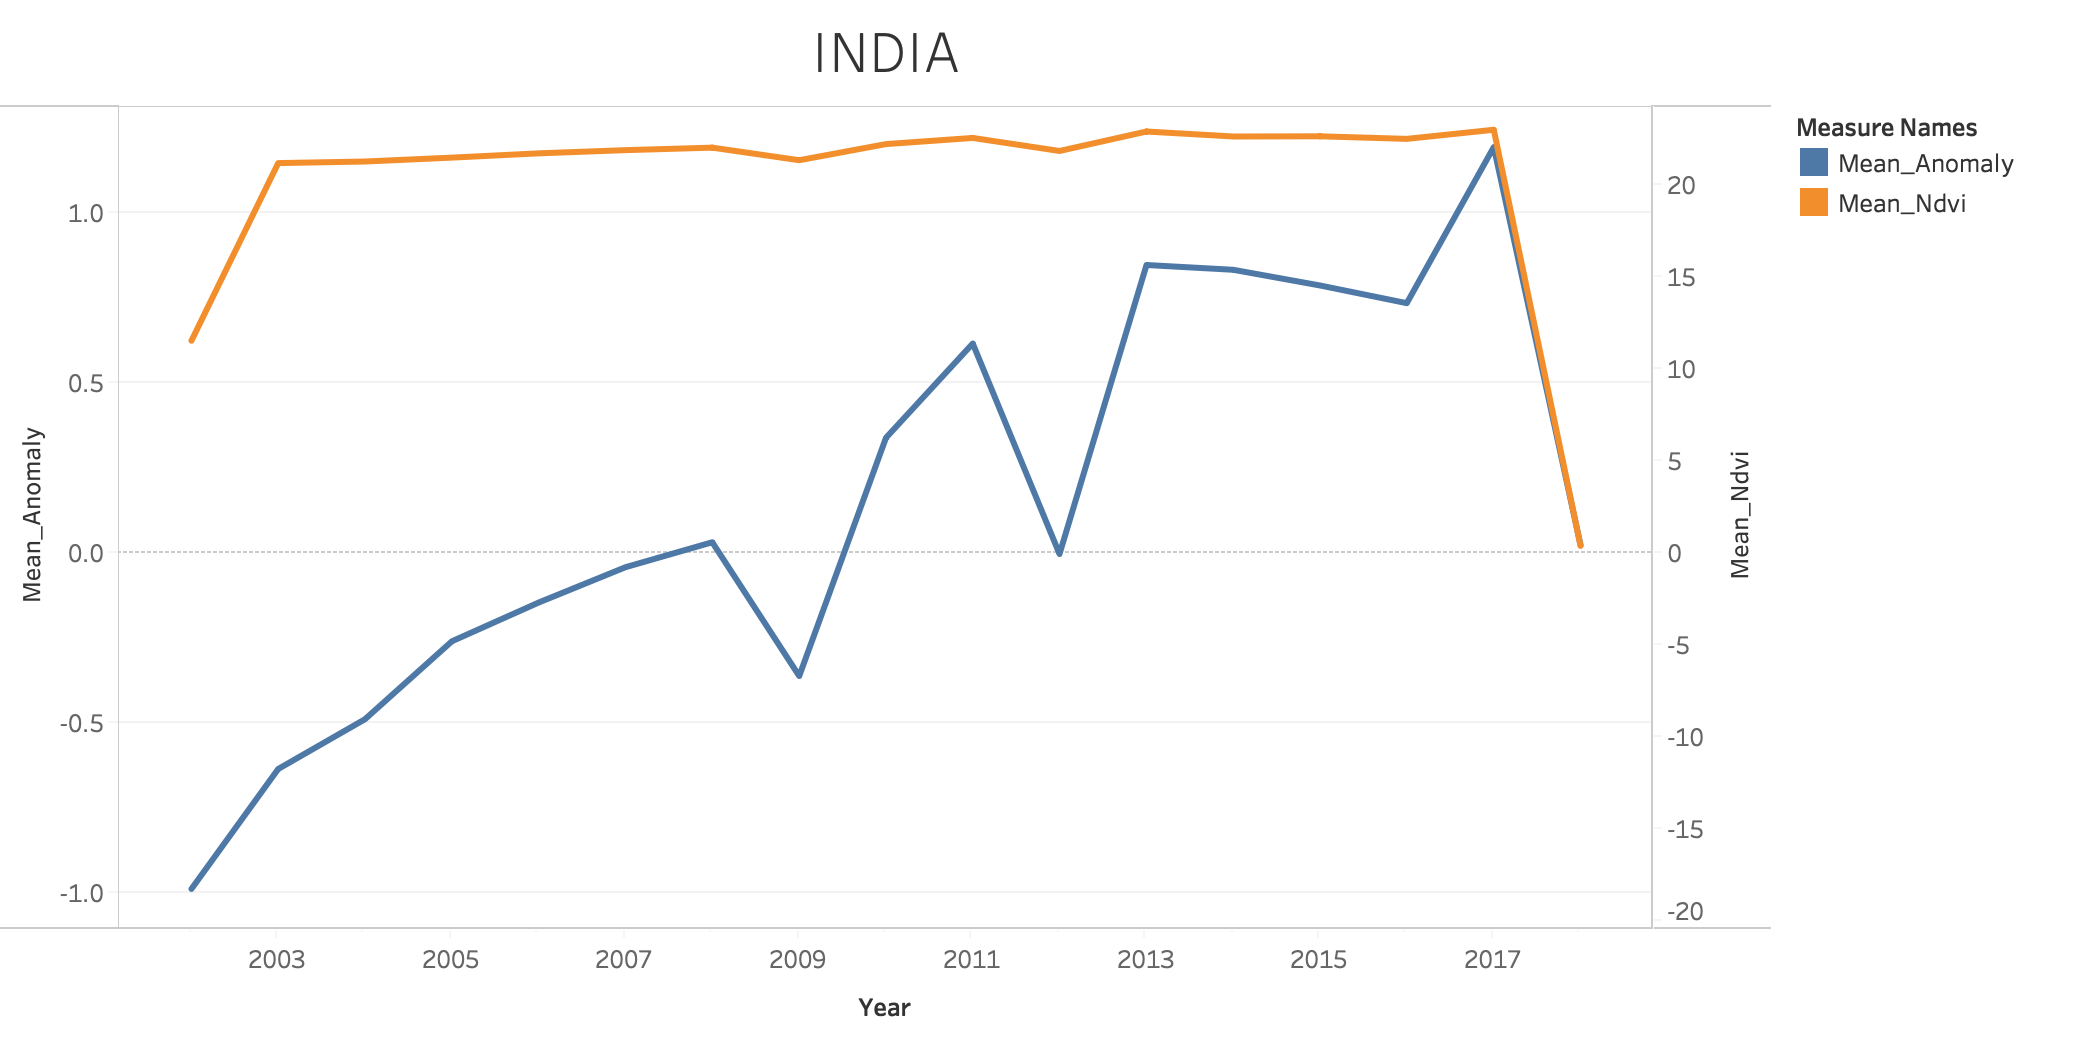
\includegraphics[width=1.0\linewidth]{figures/ch5/Mean/INDIA_mean.png}
            \caption{Mean graph - India}\label{Fig:INDIA_mean}
    \end{figure}
    
     \begin{figure}[H]
            \centering
            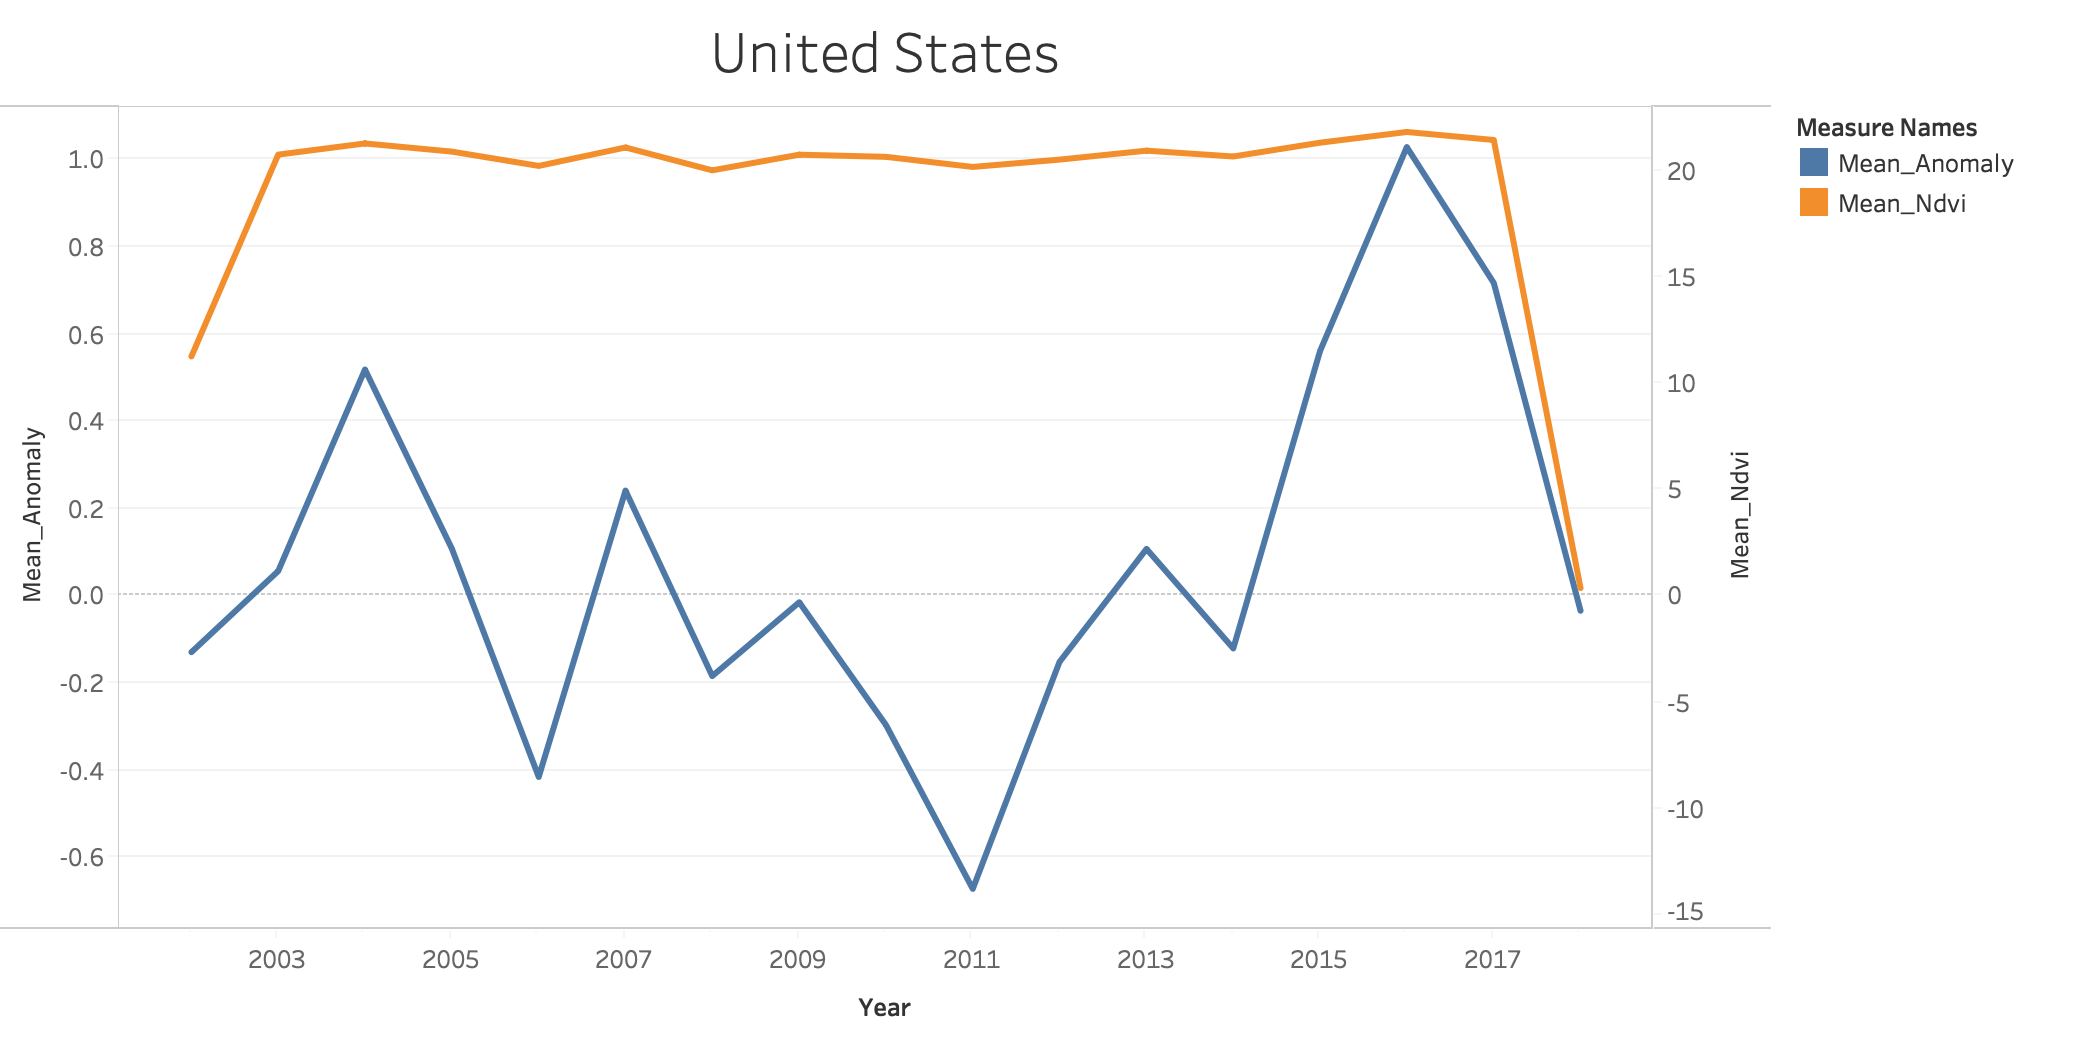
\includegraphics[width=1.0\linewidth]{figures/ch5/Mean/US_mean.png}
            \caption{\label{fig:US_mean}Mean graph - United States}
    \end{figure}

    \item \textbf{Standard Deviation NDVI \& Anomaly distribution over the years}
    
    \begin{figure}[H]
            \centering
            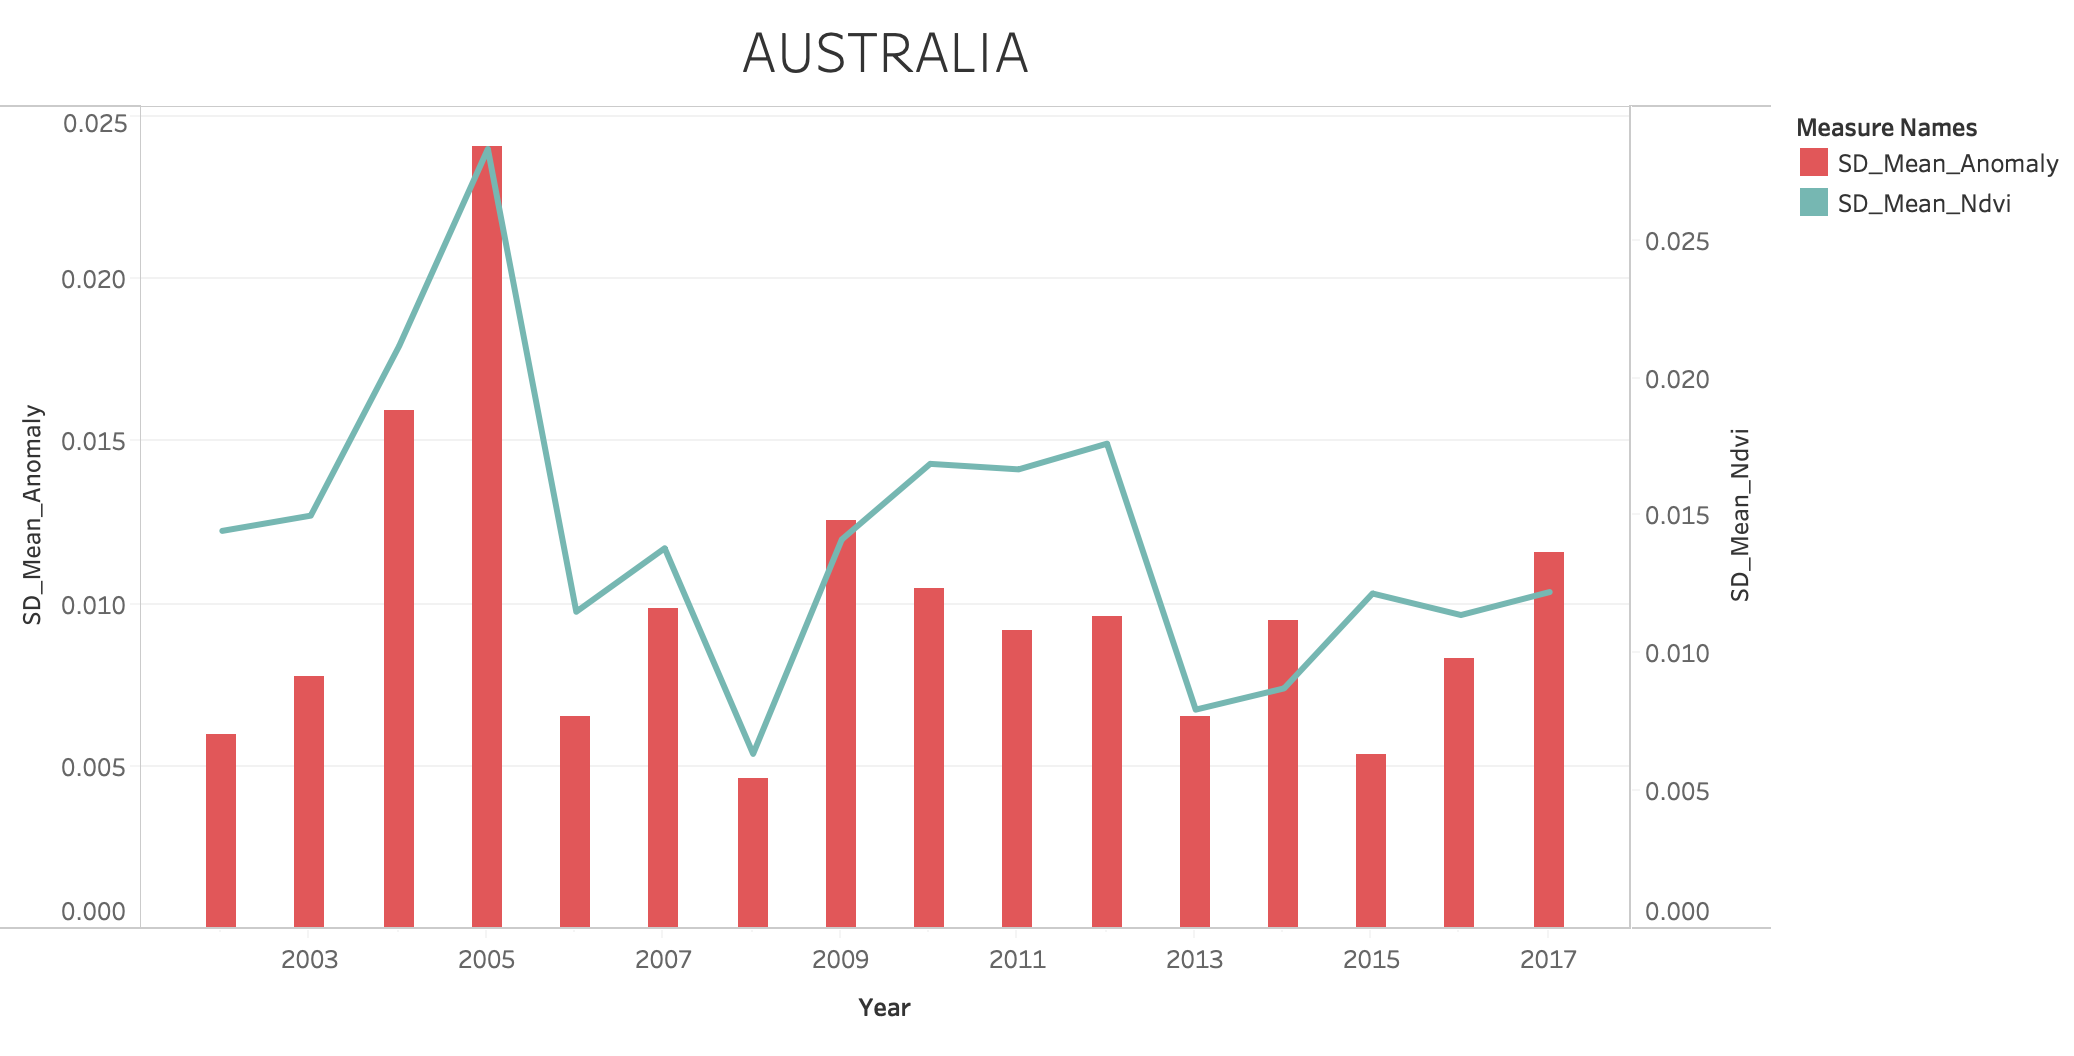
\includegraphics[width=1.0\linewidth]{figures/ch5/StandardDeviation/AUSTRALIA_SD.png}
            \caption{Standard deviation graph - Australia}\label{Fig:AUSTRALIA_SD}
    \end{figure}
    
    \begin{figure}[H]
            \centering
             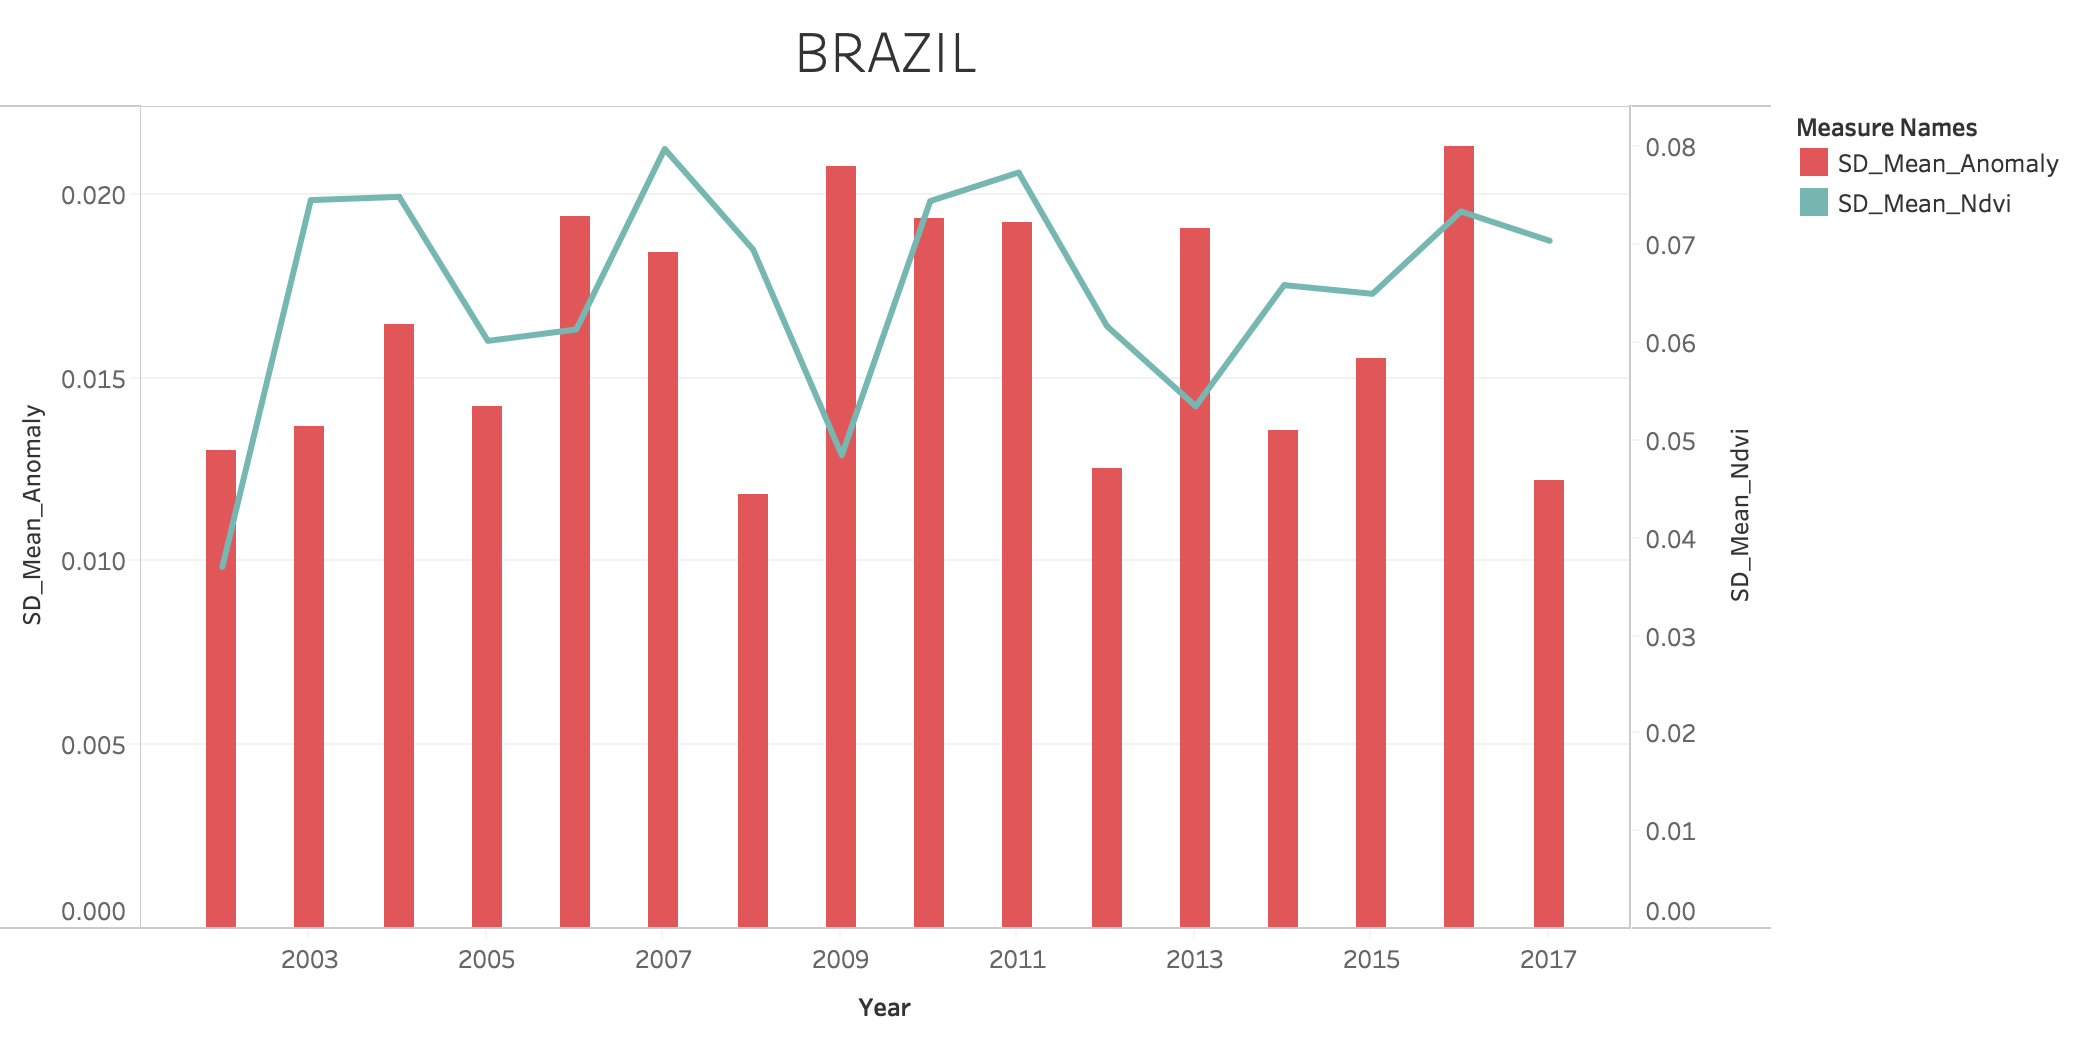
\includegraphics[width=1.0\linewidth]{figures/ch5/StandardDeviation/BRAZIL_SD.png}
            \caption{Standard deviation graph - Brazil}\label{Fig:BRAZIL_SD}
    \end{figure}
    
    \begin{figure}[H]
            \centering
            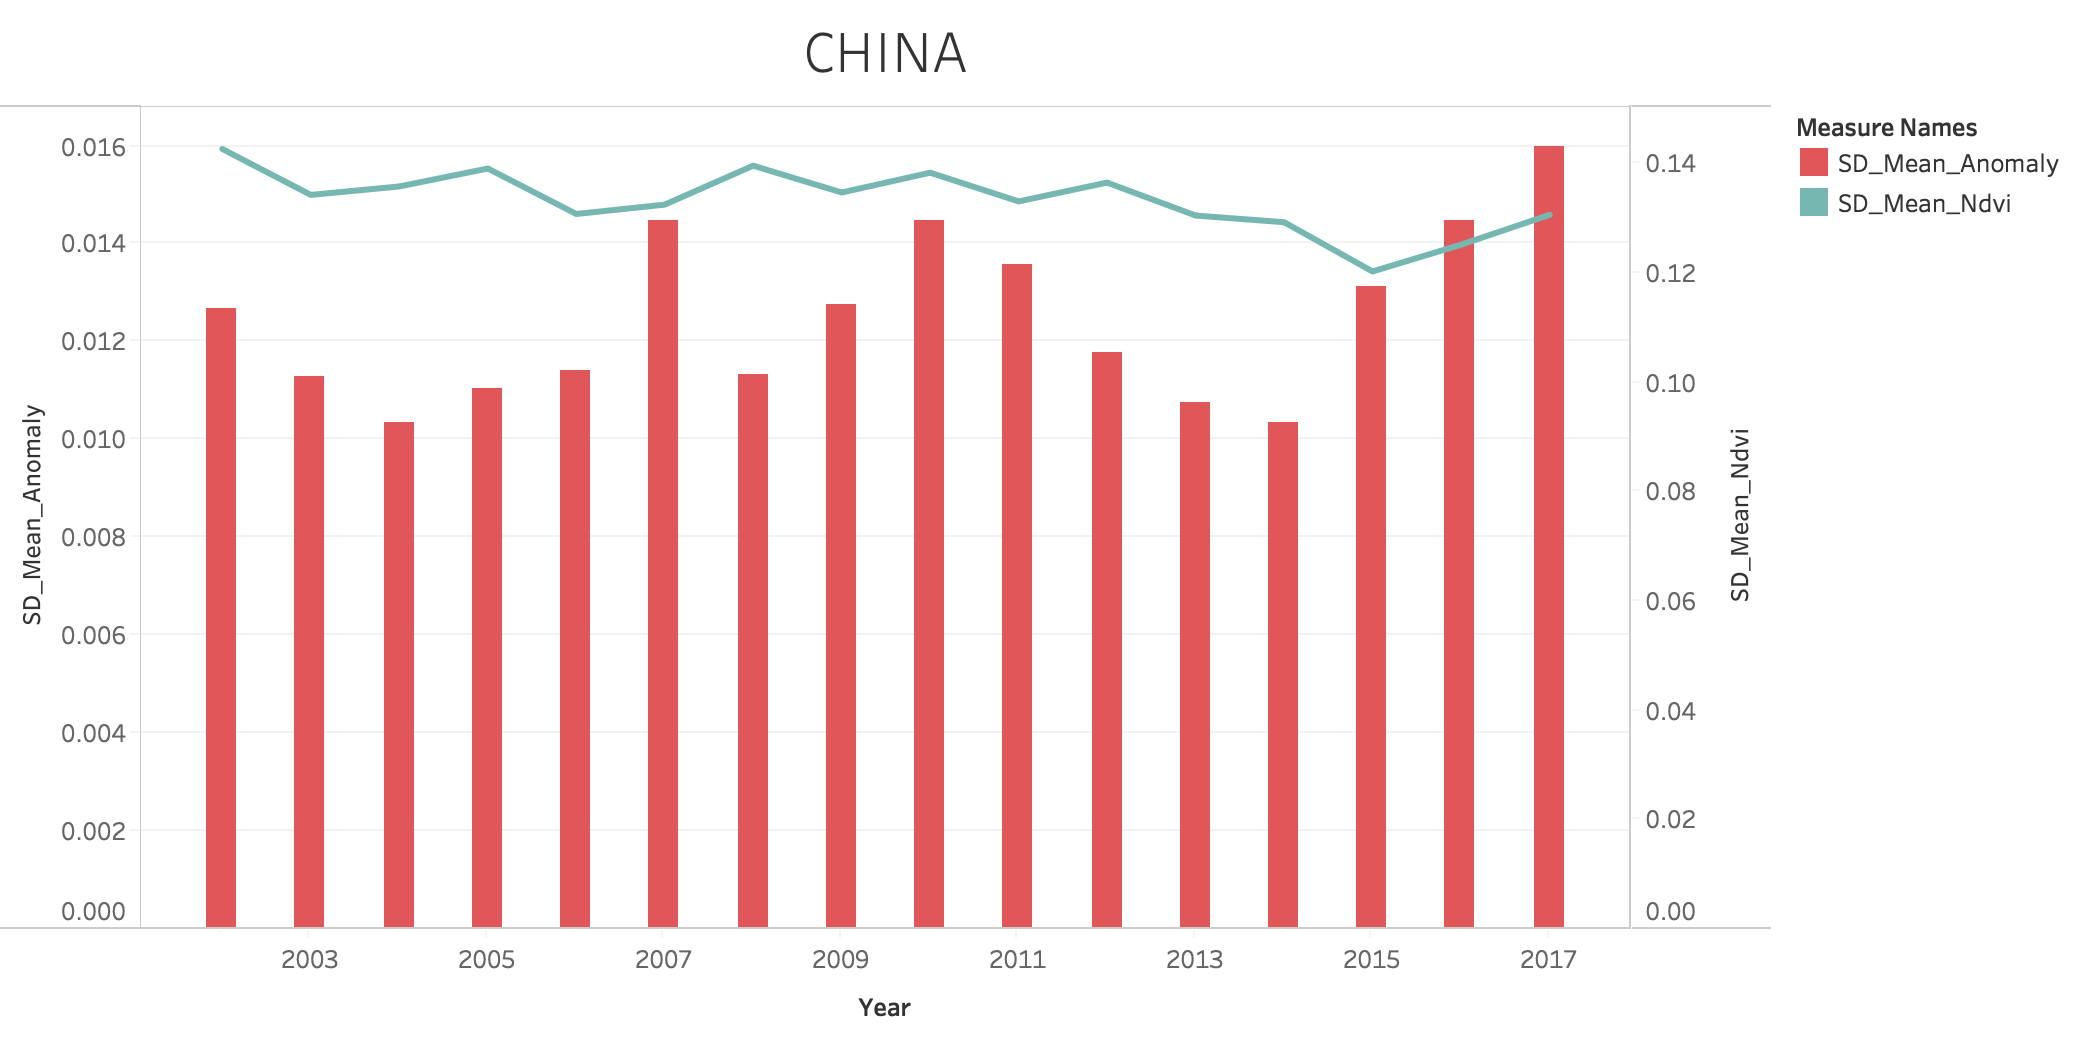
\includegraphics[width=1.0\linewidth]{figures/ch5/StandardDeviation/CHINA_SD.png}
            \caption{Standard deviation graph - China}\label{Fig:CHINA_SD}
    \end{figure}
    
    \begin{figure}[H]
            \centering
            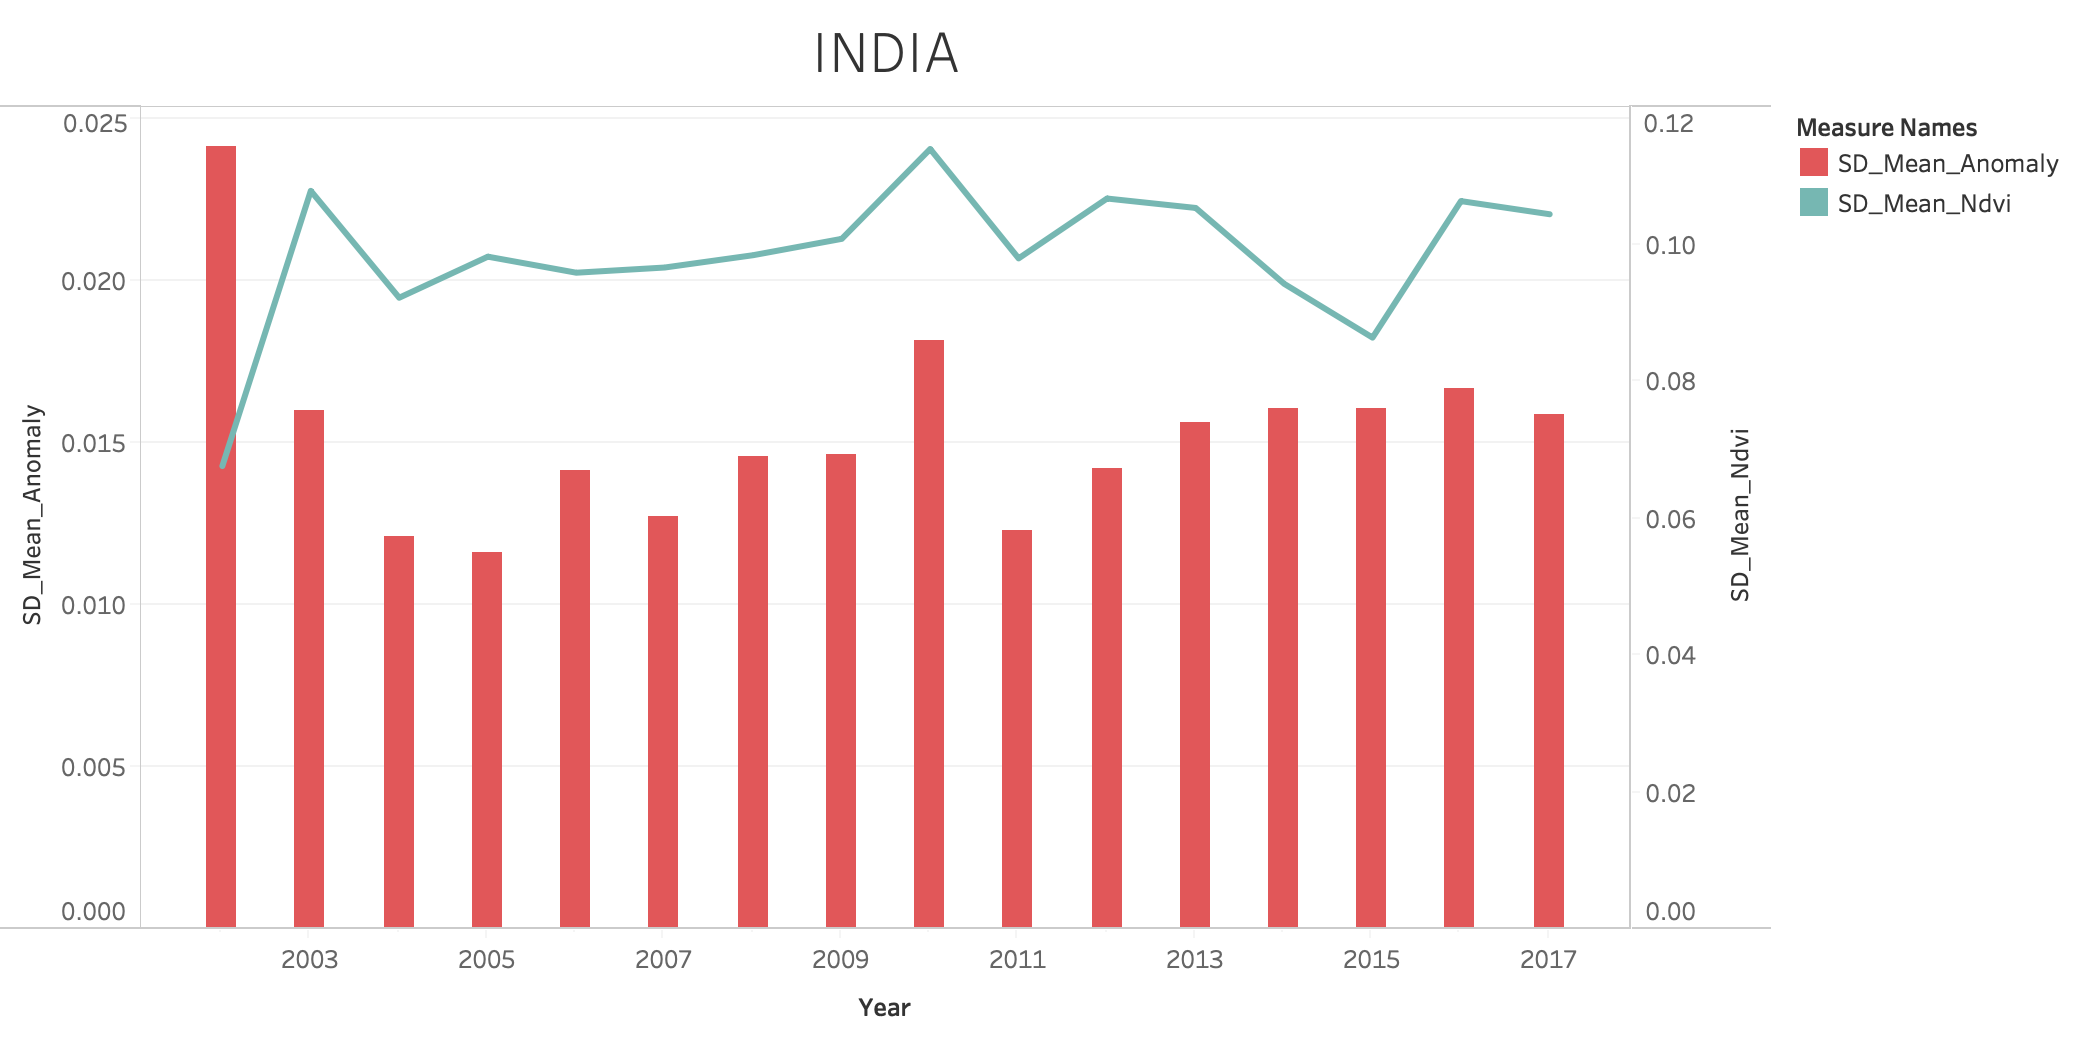
\includegraphics[width=1.0\linewidth]{figures/ch5/StandardDeviation/INDIA_SD.png}
            \caption{Standard deviation graph - India}\label{Fig:INDIA_SD}
    \end{figure}
    
     \begin{figure}[H]
            \centering
            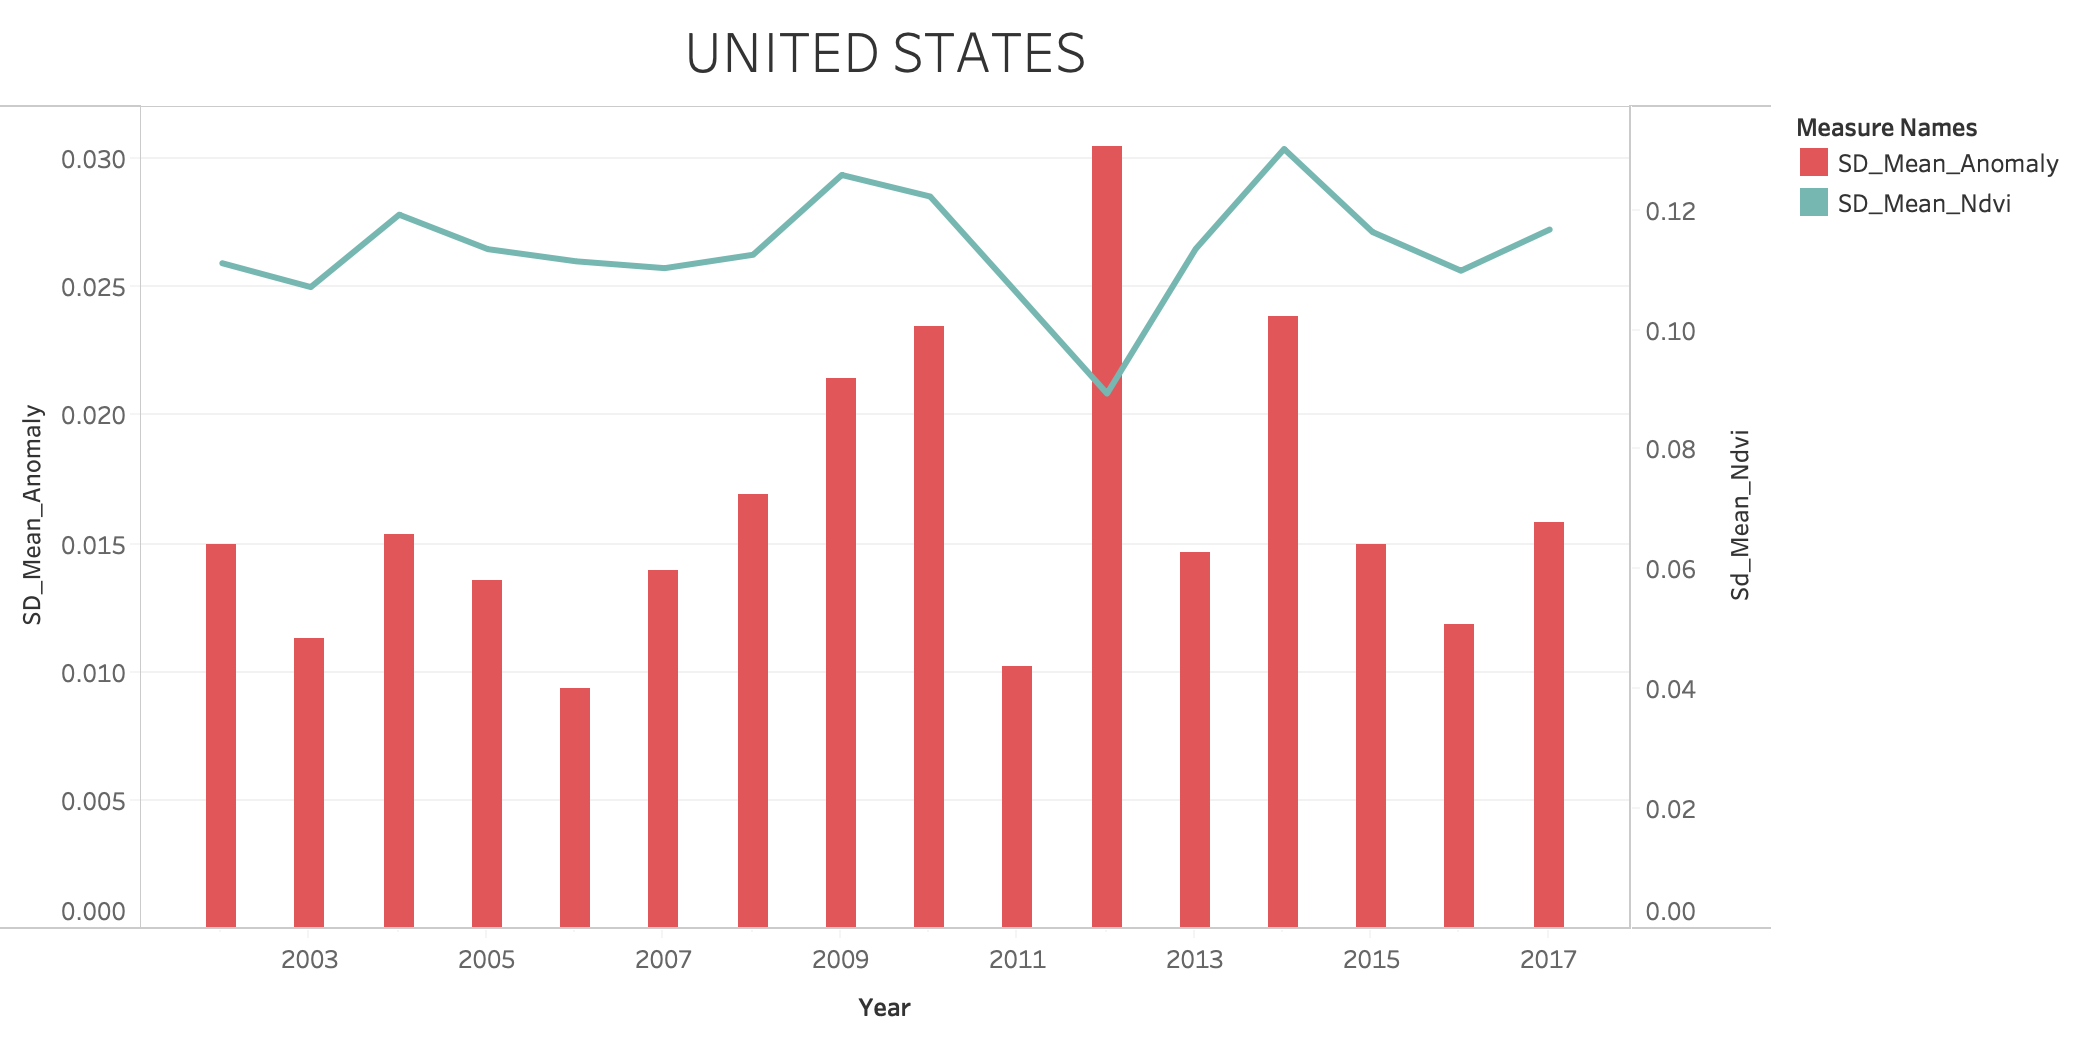
\includegraphics[width=1.0\linewidth]{figures/ch5/StandardDeviation/US_SD.png}
            \caption{\label{fig:US_SD}Standard deviation graph - United States}
    \end{figure}
   
   
    \item \textbf{Histogram NDVI \& Anomaly distribution over the years}
    
    \begin{figure}[H]
            \centering
            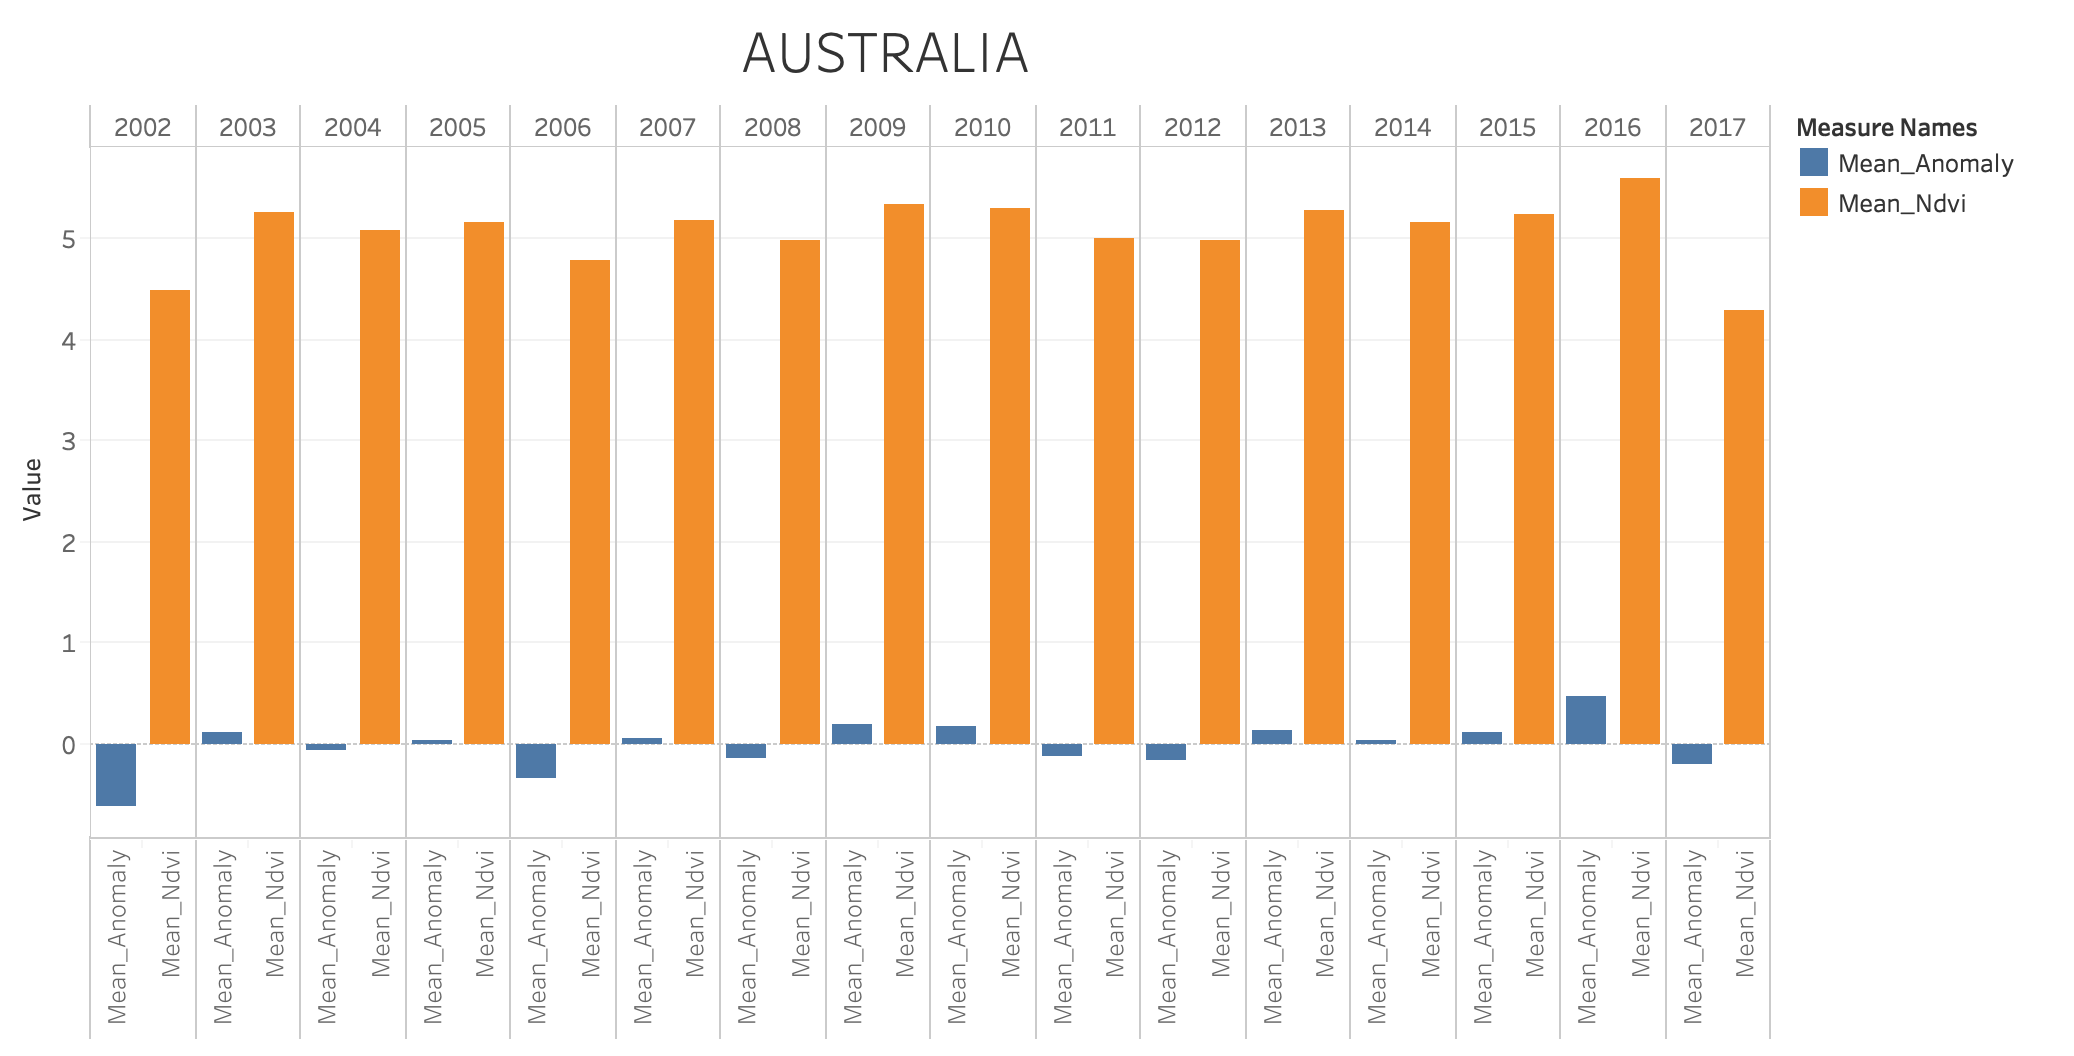
\includegraphics[width=1.0\linewidth]{figures/ch5/Histograms/AUSTRALIA_histogram.png}
            \caption{Histogram graph - Australia}\label{Fig:AUSTRALIA_histogram}
    \end{figure}
    
    \begin{figure}[H]
            \centering
            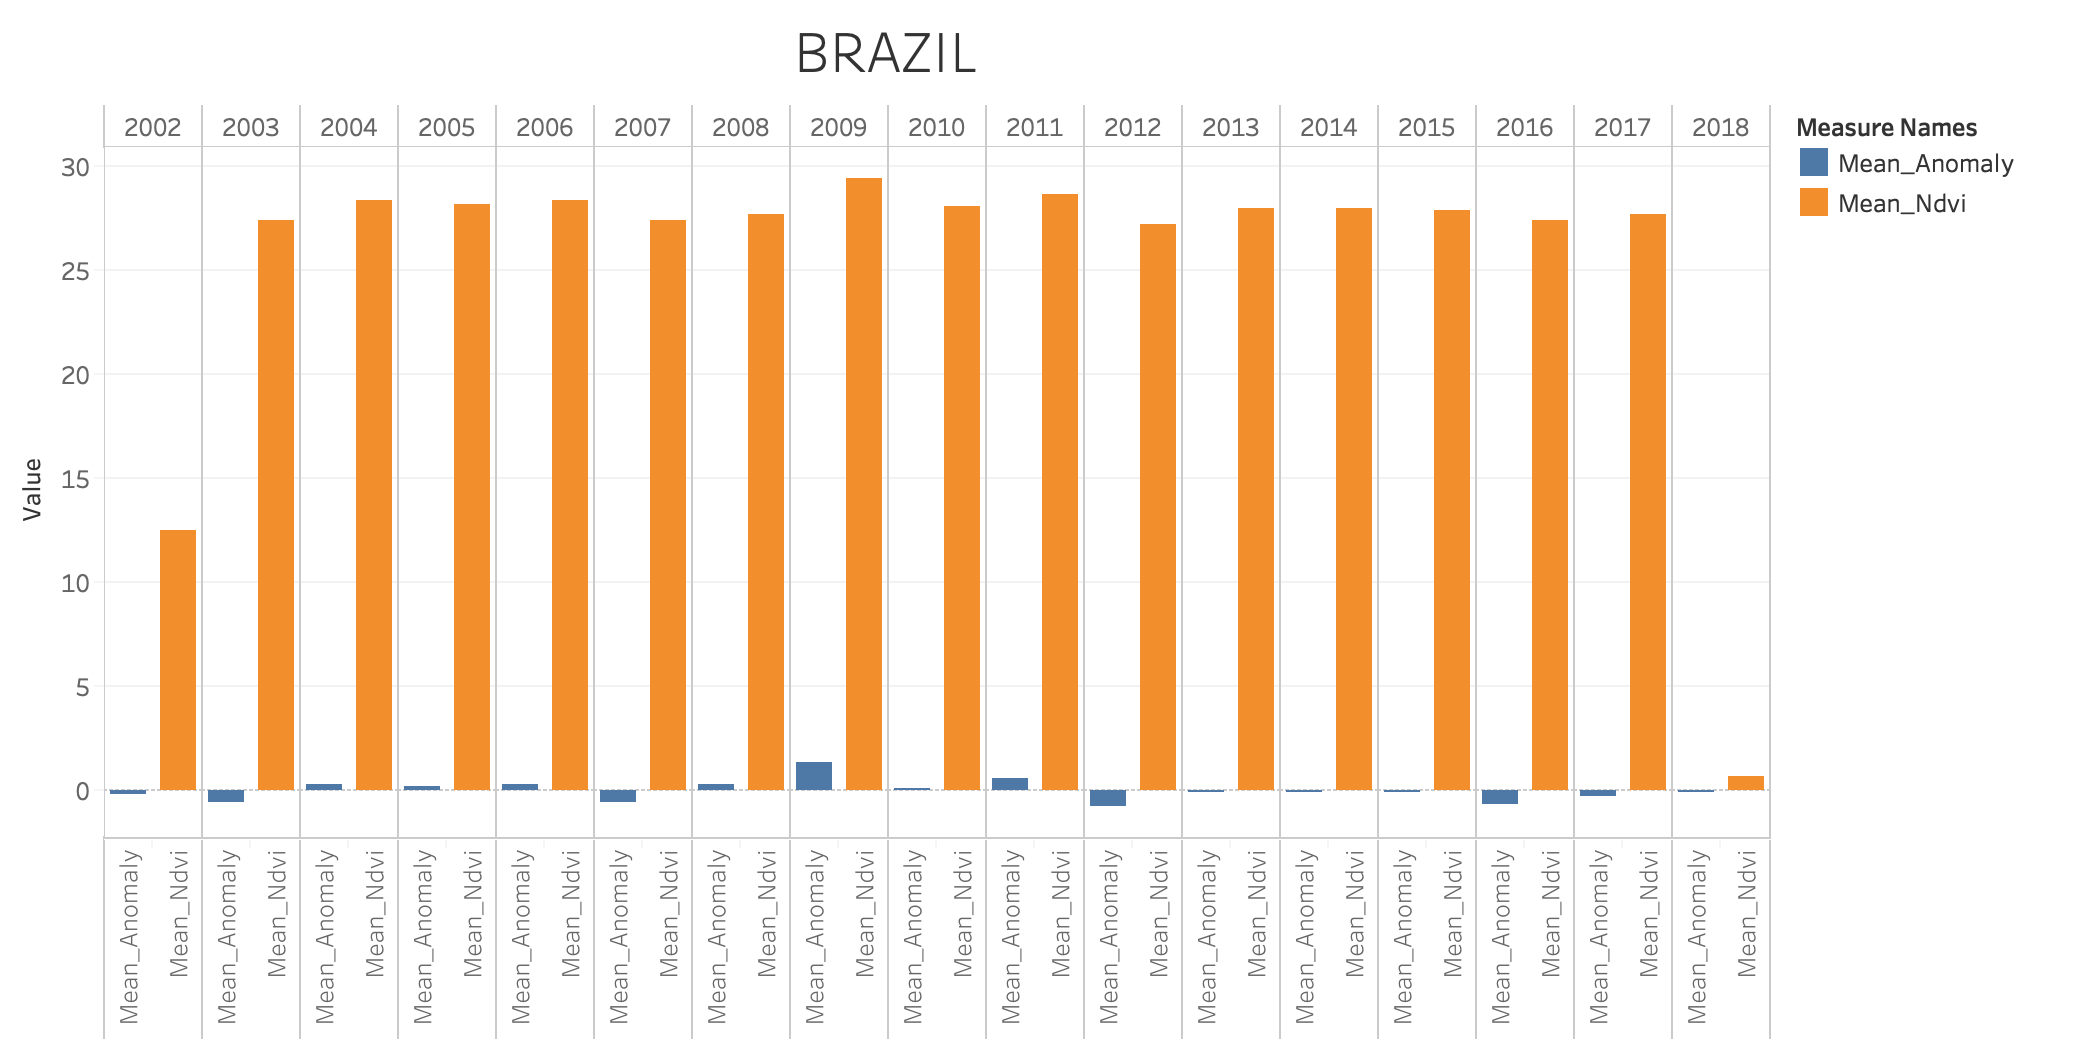
\includegraphics[width=1.0\linewidth]{figures/ch5/Histograms/BRAZIL_histogram.png}
            \caption{Histogram graph - Brazil}\label{Fig:BRAZIL_histogram}
    \end{figure}
    
    \begin{figure}[H]
            \centering
            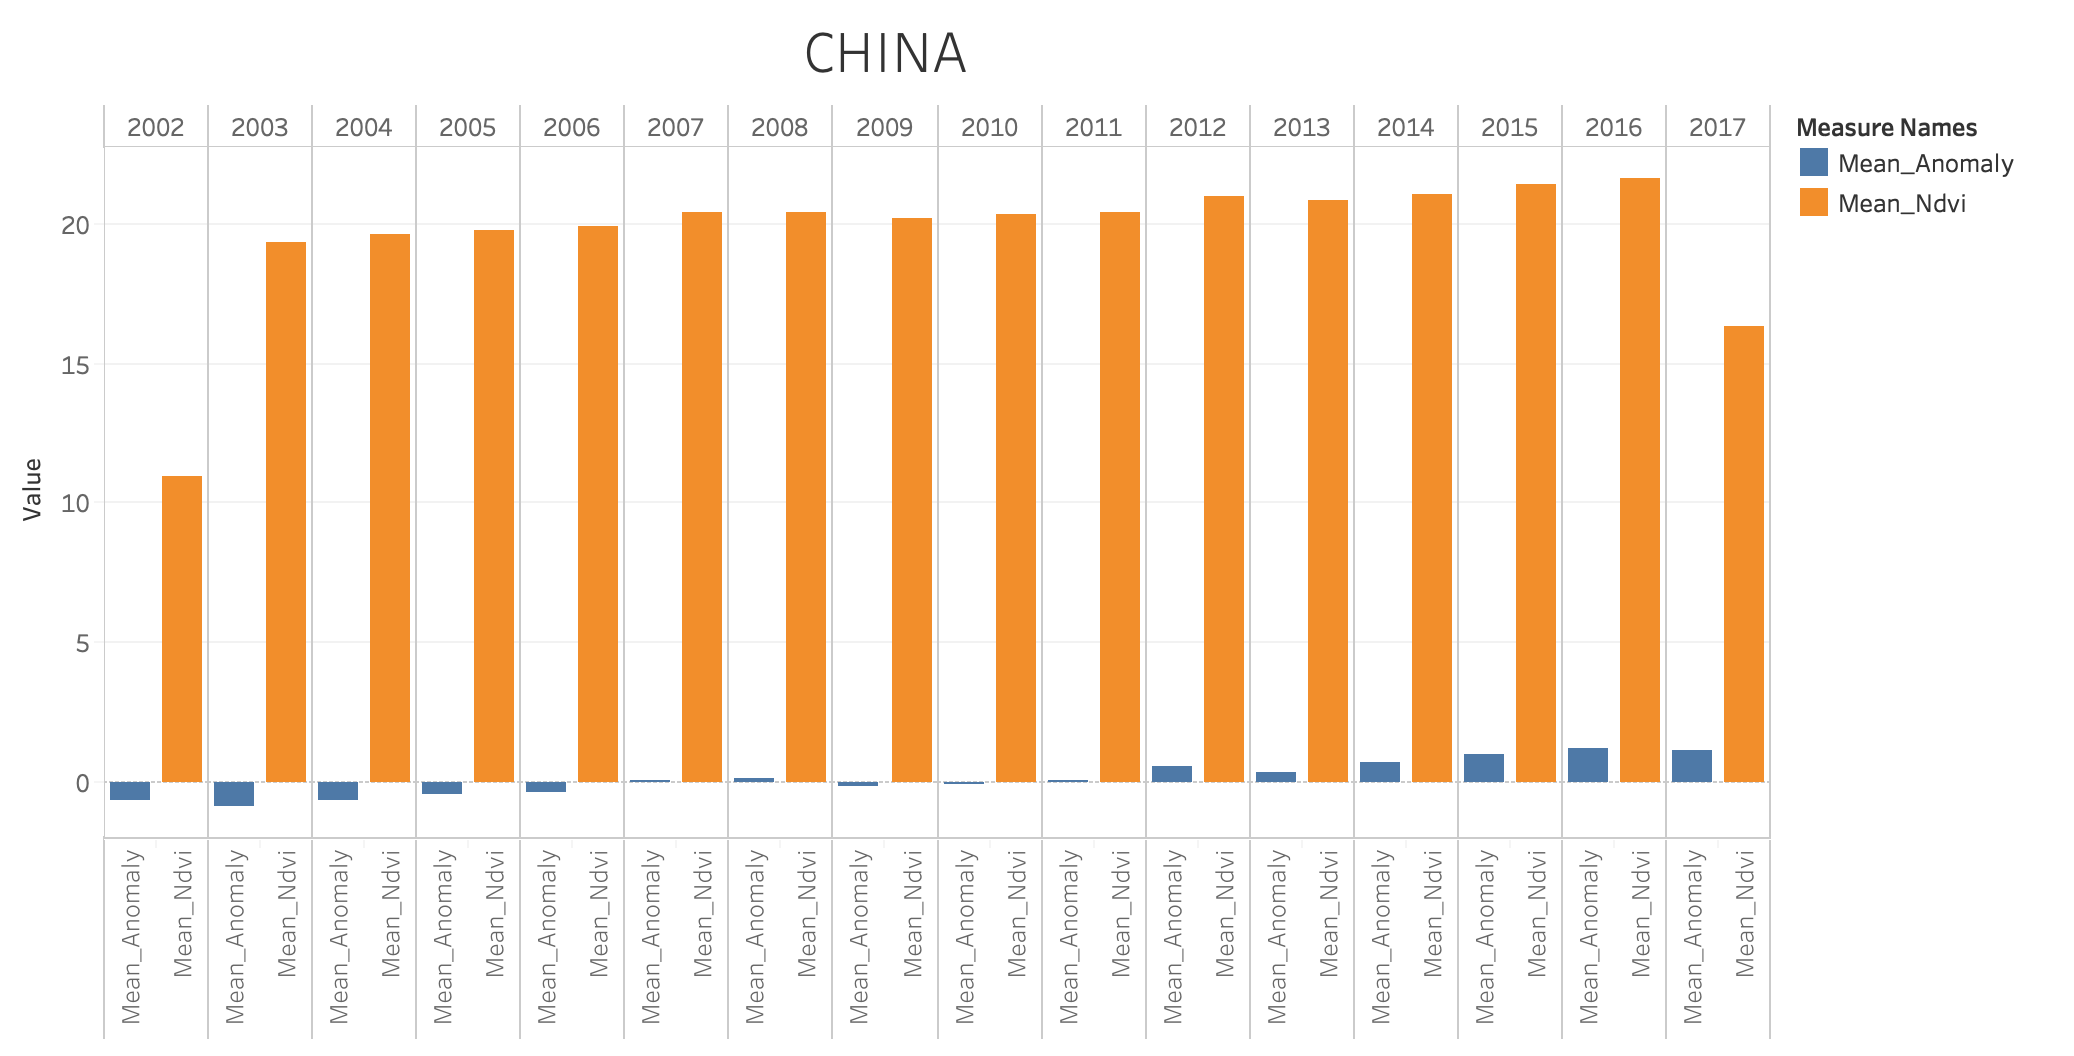
\includegraphics[width=1.0\linewidth]{figures/ch5/Histograms/CHINA_histogram.png}
            \caption{Histogram graph - China}\label{Fig:CHINA_histogram}
    \end{figure}
    
    
    \begin{figure}[H]
            \centering
            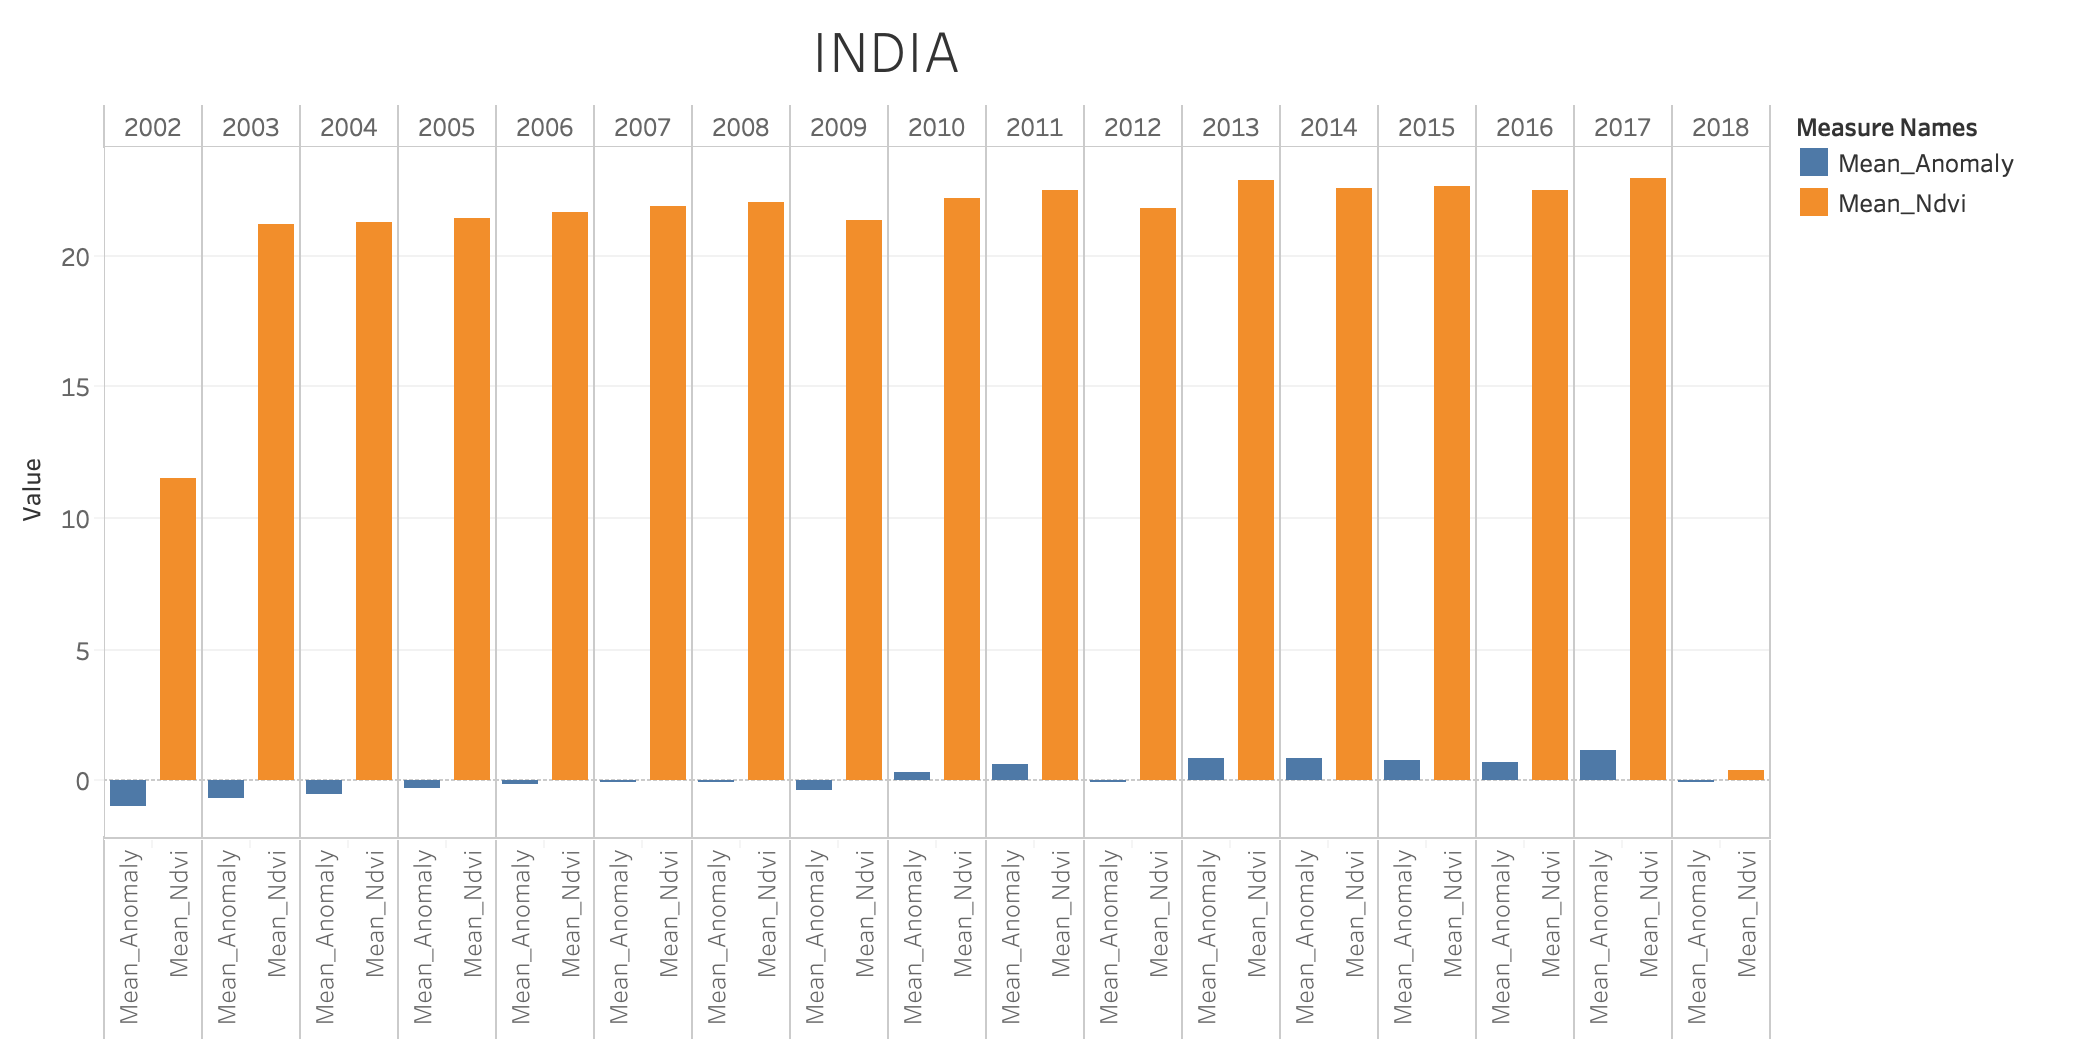
\includegraphics[width=1.0\linewidth]{figures/ch5/Histograms/INDIA_histogram.png}
            \caption{Histogram graph - India}\label{Fig:INDIA_histogram}
    \end{figure}
    
   
     \begin{figure}[H]
            \centering
            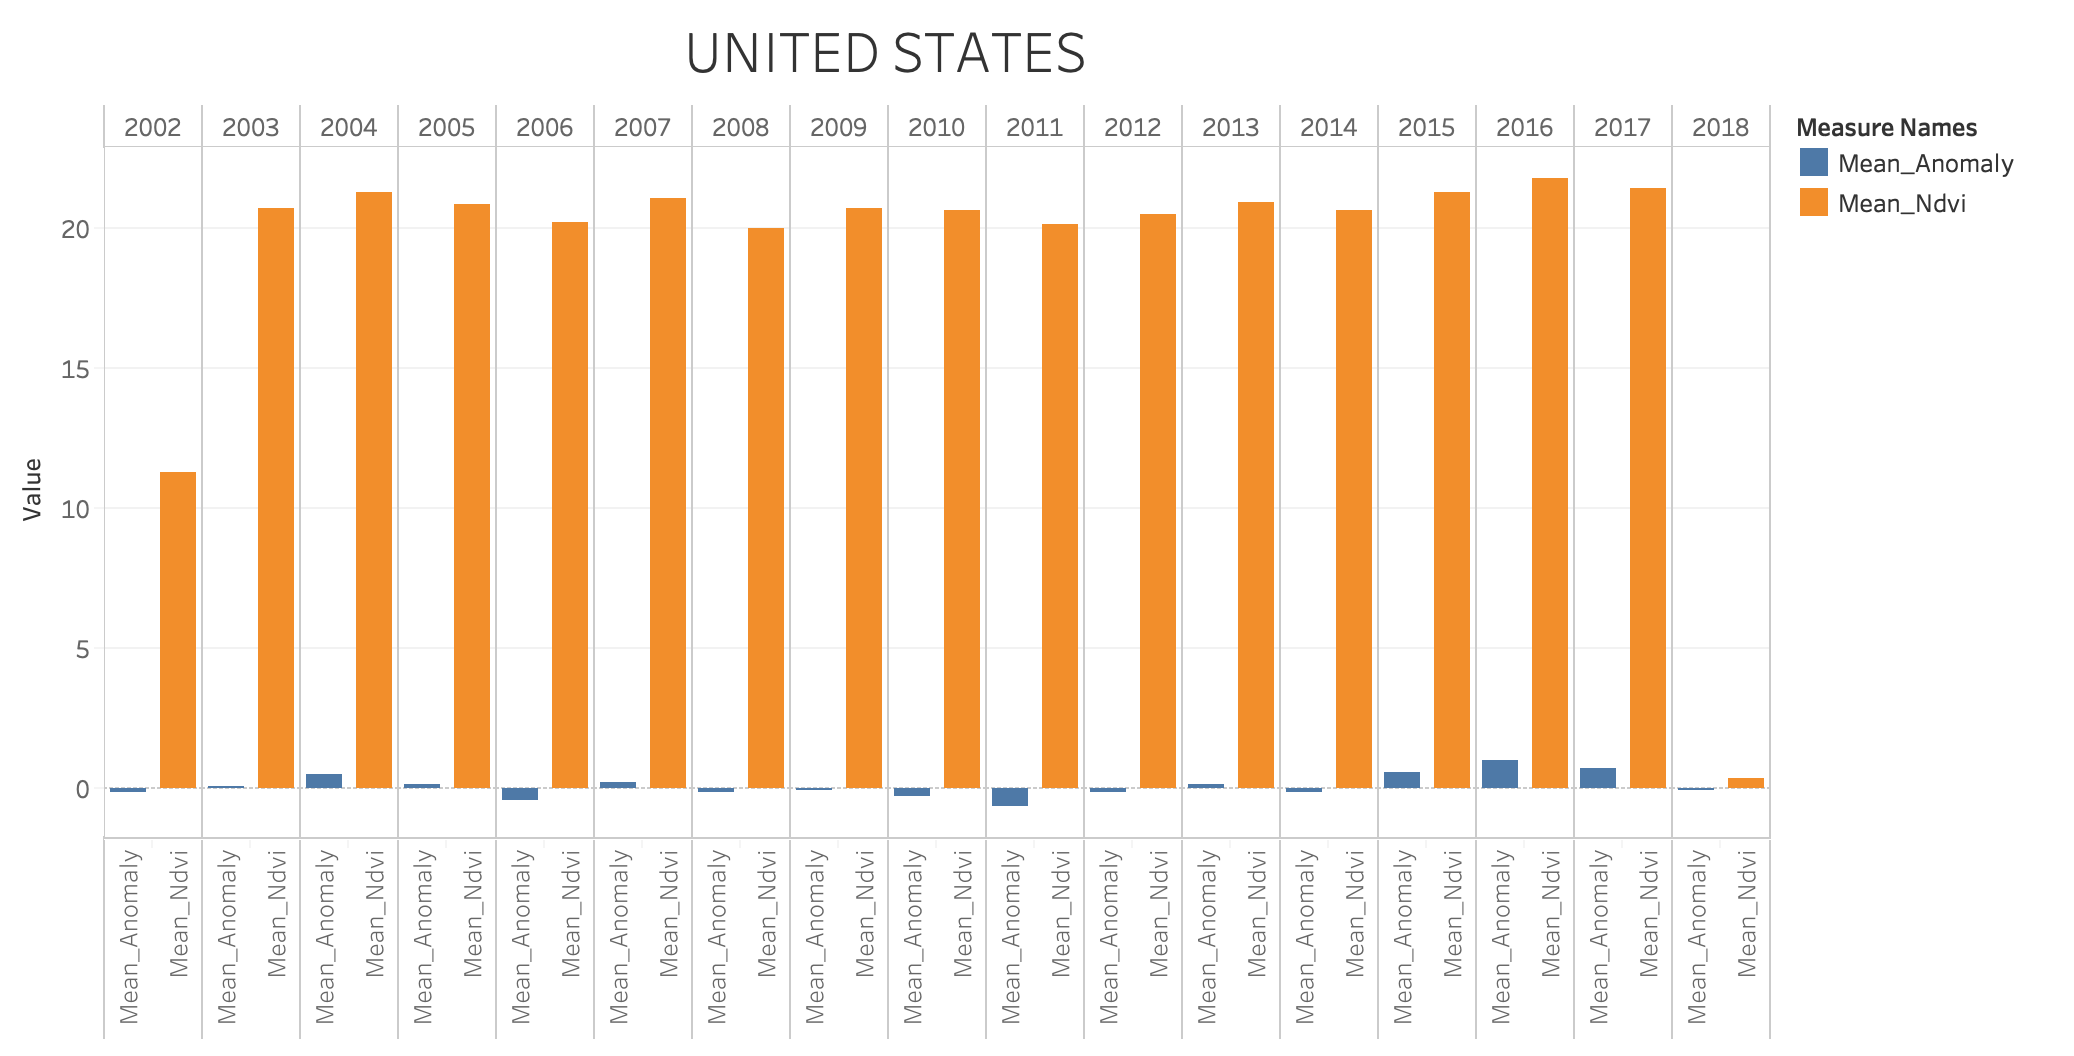
\includegraphics[width=1.0\linewidth]{figures/ch5/Histograms/US_histogram.png}
            \caption{\label{fig:US_histogram} Histogram graph - United States}
    \end{figure}


\end{itemize}

\section{SVD Analysis}

\gls{svd} is the overview of the eigen decomposition of a positive semidefinite normal matrix to any $m$ x $n$ matrix through a calculation of the polar breakdown. It has numerous practical functions in signal processing, statistics, and data analysis.
One way to visualize SVD is by considering what happens to the unit sphere in the vector space as it’s being transformed. Transformation creates a rotation if a matrix has orthonormal rows. A scaling process is also taking place, followed by a rotation. Any transformation can be expressed as a rotation followed by a scaling and by an additional rotation \cite{SVD}.

\begin{equation} \label{eq:svd_formula}
 A = UDV^{T}
\end{equation}

Equation 5.3 show "SVD" mathematical expression where $A$ is $m$ x $n$ real matrix with $m>n$, $U$ with dimensions $m$ x $m$ and $V$ with dimensions $n$ x $n$. Figure~\ref{fig:svd_matrix} shows visualization of the matrix multiplications in \gls{svd}.

    \begin{figure}[H]
            \centering
            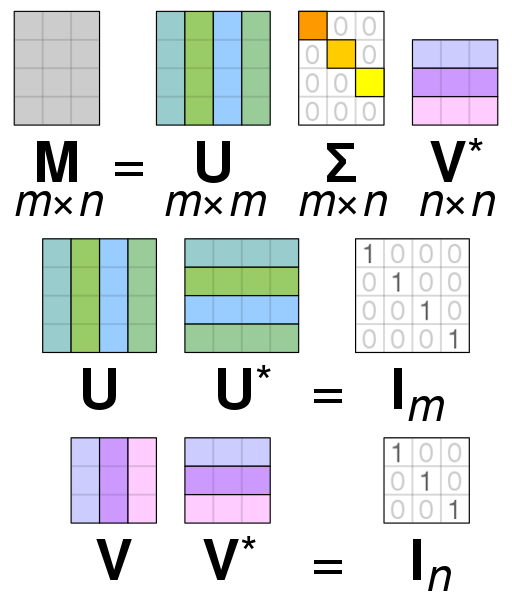
\includegraphics[width=0.5\linewidth]{figures/ch5/svd_matrix.png}
            \caption{\label{fig:svd_matrix} Matrix multiplications in SVD shown visually \cite{SVD}}
    \end{figure}

As an application, SVD is utilized to perform principle component analysis (PCA) that intends to decompose a matrix with the end goal to discover the directions (called principal axes). It also tells about the directions in which the data is distributed and is useful for dimensionality reduction. 

Steps involved in the process of implementing \gls{svd} are as follows.

\begin{itemize}
    \item Conversion of \gls{json} \gls{ndvi} fetched data from server into a formatted \gls{csv} file on the client side.
    \item Load the csv file in R code and remove invalid or null entries with 0.
    \item Remove the states which we don't have the data for.
    \item Plot the eigen values of \gls{ndvi} covariance matrix.
    \item Implement \gls{svd} on the matrix.
    \item Plot first five \gls{eof}'s and \gls{pca}'s.
\end{itemize}

Figure~\ref{fig:svd_data_snapshot} shows the portion of mean \gls{ndvi} data that has been used for the analysis.

  \begin{figure}[H]
            \centering
            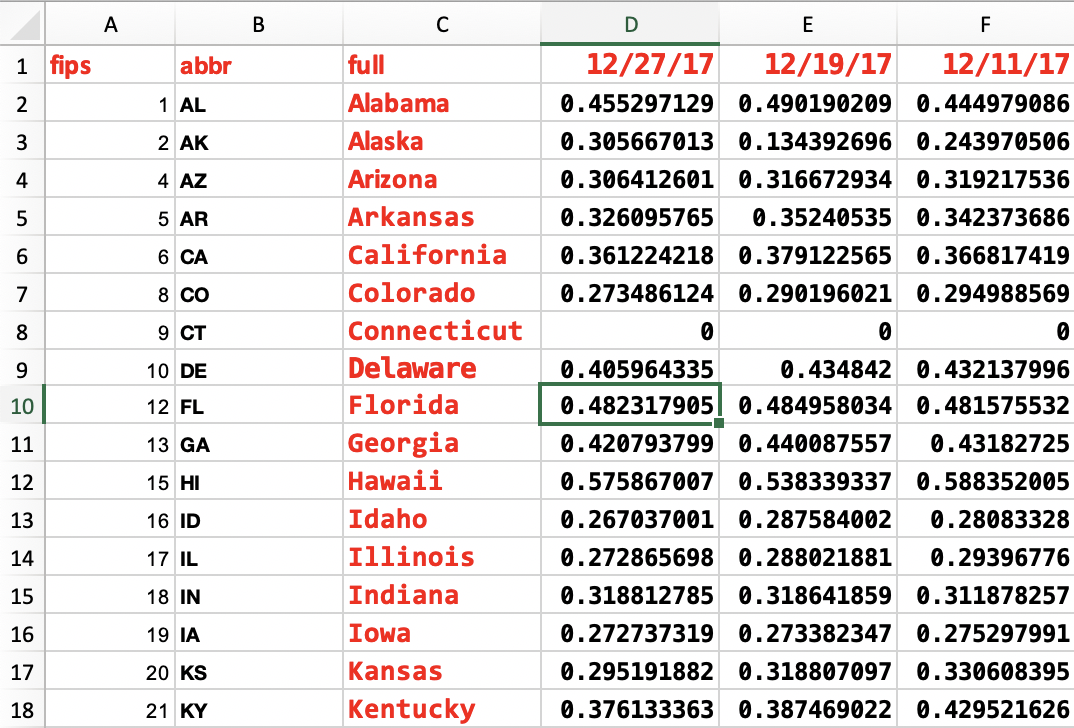
\includegraphics[width=0.9\linewidth]{figures/ch5/svd_data_snapshot.png}
            \caption{\label{fig:svd_data_snapshot} Snapshot of United States mean NDVI data of all years represented state wise}
    \end{figure}
    
\begin{figure}[H]
            \centering
            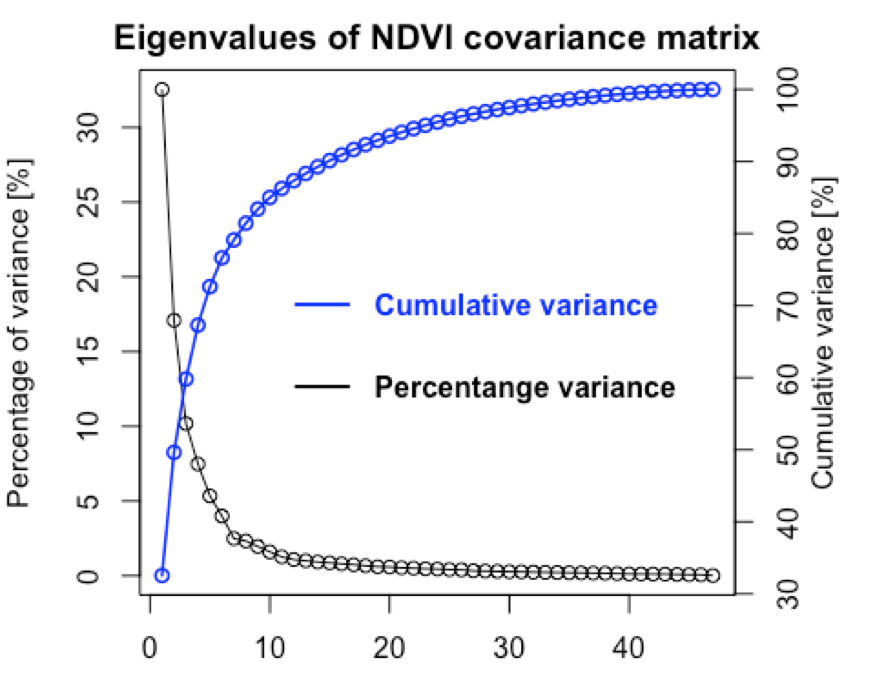
\includegraphics[width=0.70\linewidth]{figures/ch5/SVD/covarianceeigen.png}
            \caption{\label{fig:covriance} Eigen values of NDVI covariance matrix.}
    \end{figure}
    
Figure~\ref{fig:covriance} shows that within the first few modes of the curve, a big change can be observed in both the cumulative variance and the percentage variance going from about 0 to 17 and from about 32 to 10 respectively, notice that the values get smaller at the extremes, causing the points to overlap in the presence of noise.  \\
The size of $A$ matrix is $47$ x $714$, column belongs to dates and row for states. After applying \gls{svd} to matrix $A$, the matrices, $U$, $D$ and $VT$ are shown below in Figure~\ref{fig:svd_result_matrices}.

    \begin{figure}[H]
            \centering
            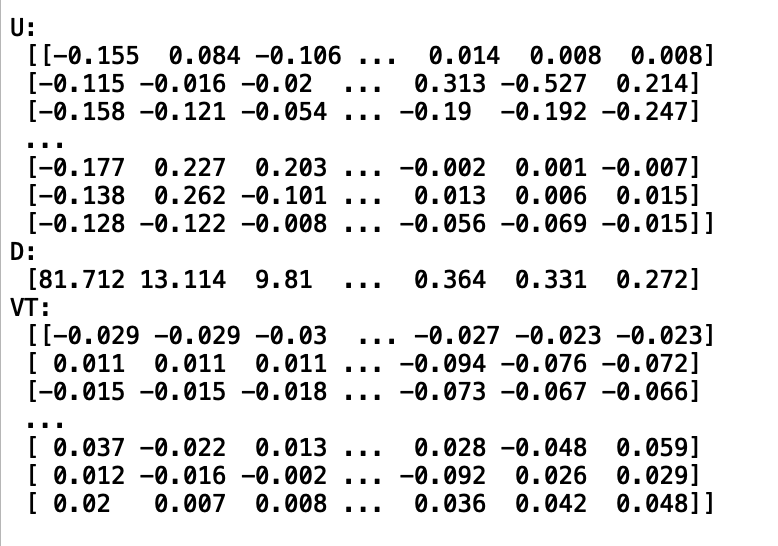
\includegraphics[width=0.70\linewidth]{figures/ch5/svd_result_matrix.png}
            \caption{\label{fig:svd_result_matrices} Result of SVD on matrix A - U, D \& VT}
    \end{figure}
    
    \gls{eof}s and \gls{pca}s plots of first five vectors has been shown in below figures.
    
     \begin{figure}[H]
            \centering
            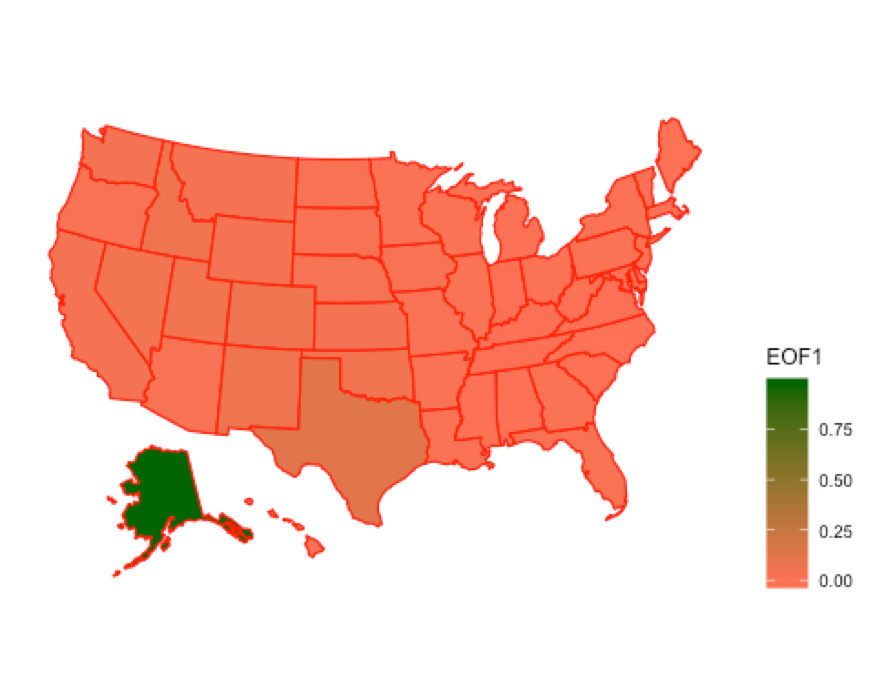
\includegraphics[width=0.70\linewidth]{figures/ch5/SVD/eof1.png}
            \caption{\label{fig:EOF_1} Mask mapping state wise of U1 vector of matrix U}
    \end{figure}
    
    Figure~\ref{fig:EOF_1} shows the mask mapping of state wise anomaly values, notice that there is little to no change in the continental US, while Alaska shows the highest value.
    
     \begin{figure}[H]
            \centering
            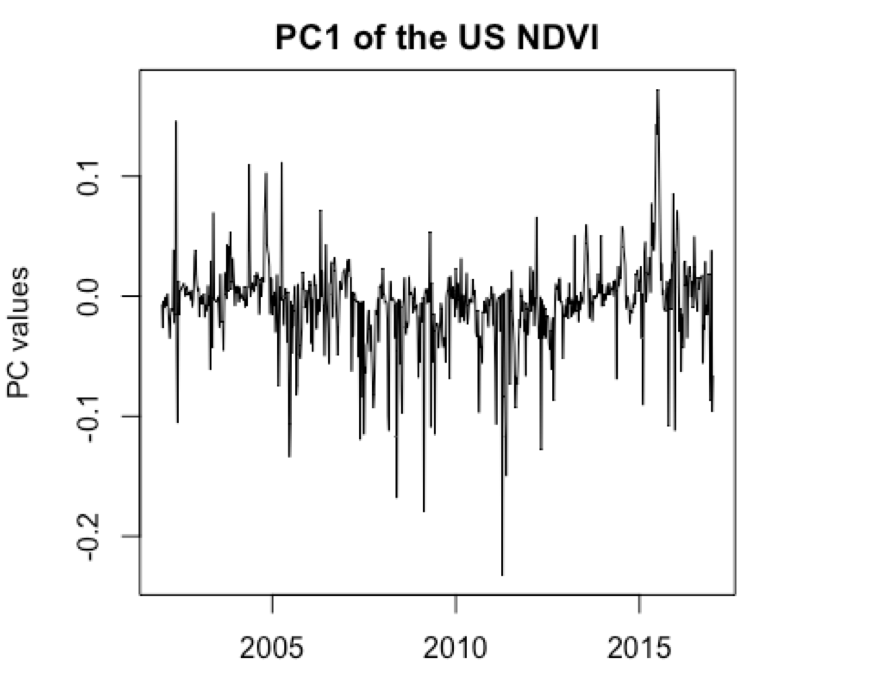
\includegraphics[width=0.70\linewidth]{figures/ch5/SVD/pc1.png}
            \caption{\label{fig:V_1} Time series analysis of V1 vector of matrix V}
    \end{figure}
    
    Figure~\ref{fig:V_1} describes extreme local minimums in 2002, 2005, 2007, 2008, 2013, 2016, and a global maximum in 2012. Local maximums are shown in 2002, 2006, 2007, 2009, and a global maximum in 2015. 
    
    \begin{figure}[H]
            \centering
            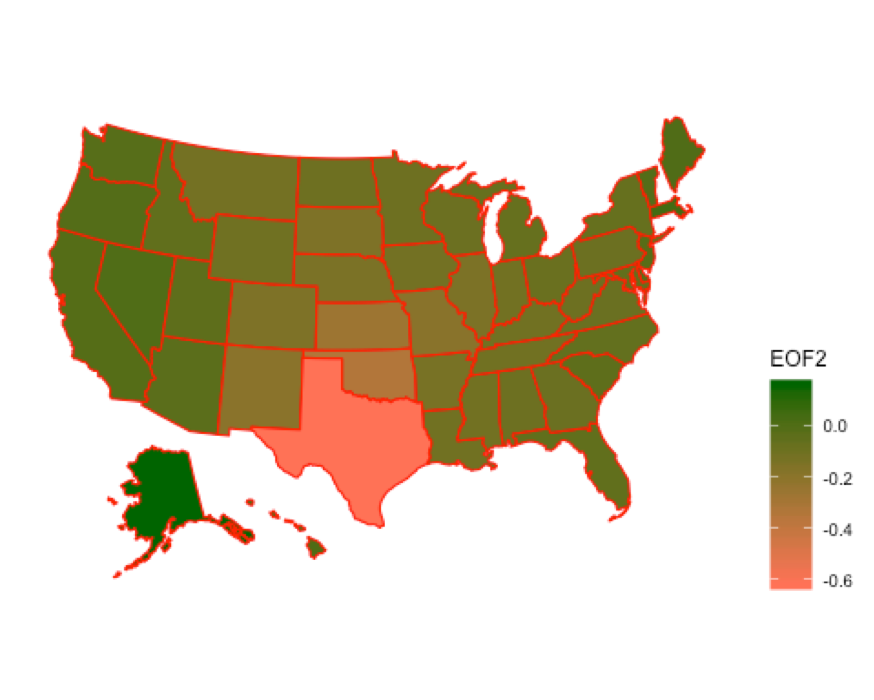
\includegraphics[width=0.70\linewidth]{figures/ch5/SVD/eof2.png}
            \caption{\label{fig:EOF_2} Mask mapping state wise of U2 vector of matrix U}
    \end{figure}
    
     Figure~\ref{fig:EOF_2} shows the east and west patters as positive indicating close to zero anomaly, on the other hand the mountain region shows the opposite, the values are on the negative side.
    
    \begin{figure}[H]
            \centering
            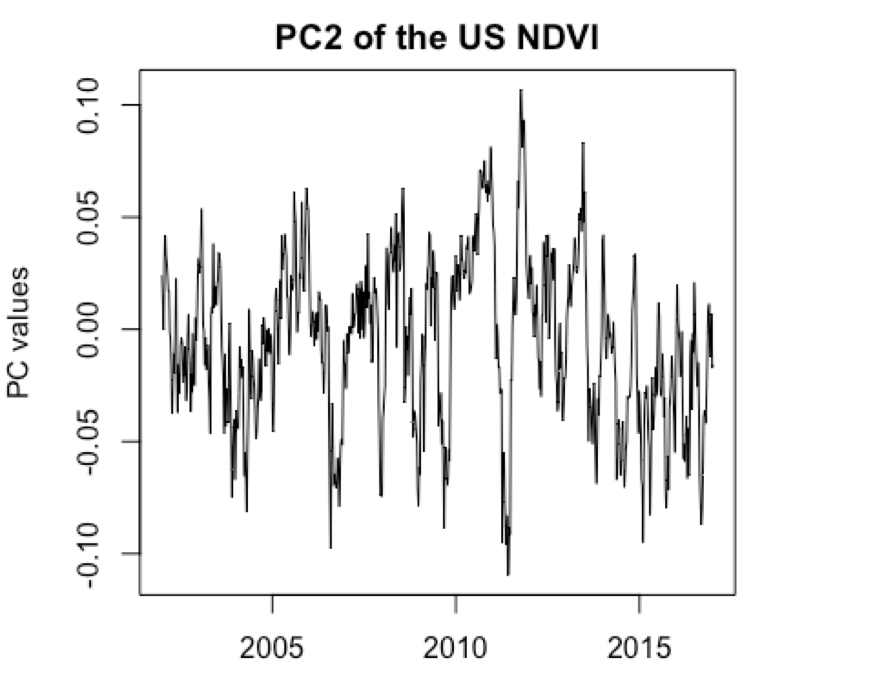
\includegraphics[width=0.70\linewidth]{figures/ch5/SVD/pc2.png}
            \caption{\label{fig:V_2} Time series analysis of V2 vector of matrix V}
    \end{figure}
    
    Figure~\ref{fig:V_2} shows an increase and then a sudden drop around 2005, 2010 and 2015 showing an interesting pattern in the anomaly.
    
     \begin{figure}[H]
            \centering
            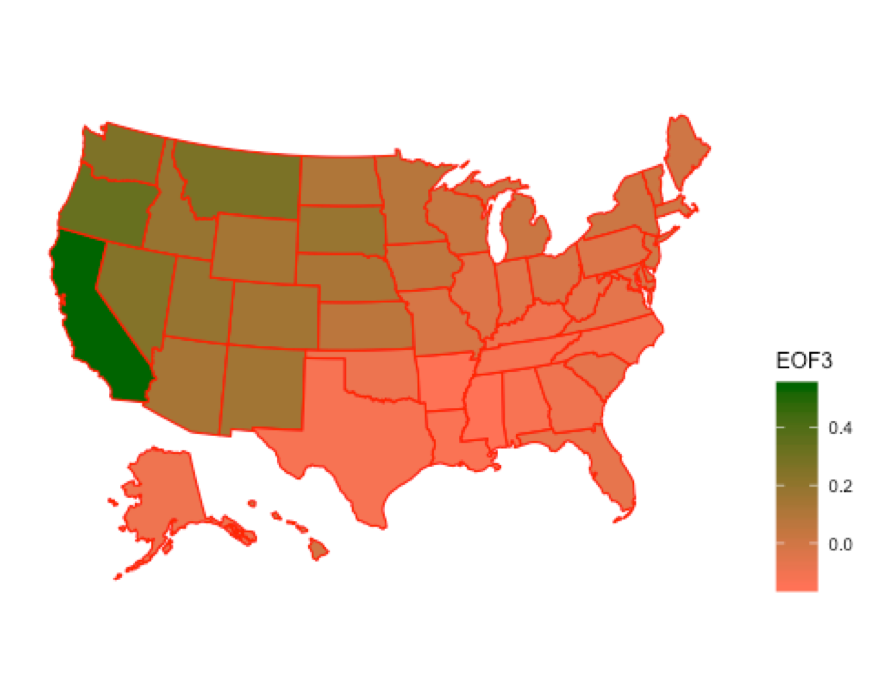
\includegraphics[width=0.70\linewidth]{figures/ch5/SVD/eof3.png}
            \caption{\label{fig:EOF_3} Mask mapping state wise of U3 vector of matrix U}
    \end{figure}
    
   Figure~\ref{fig:EOF_3} shows the southeast area with almost zero to negative anomaly, while northwest shows the opposite.
    
     \begin{figure}[H]
            \centering
            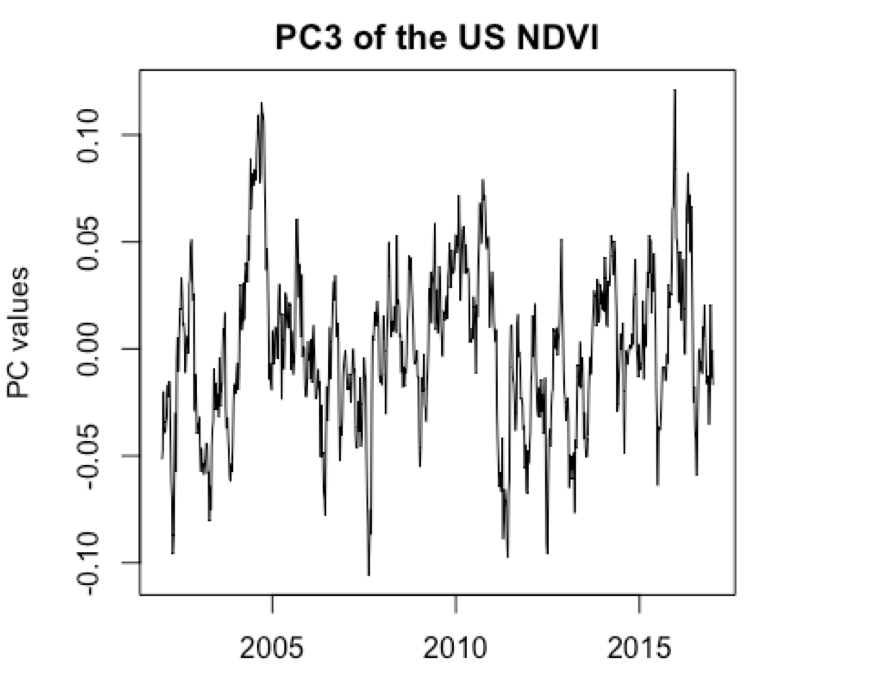
\includegraphics[width=0.70\linewidth]{figures/ch5/SVD/pc3.png}
            \caption{\label{fig:V_3} Time series analysis of V3 vector of matrix V}
    \end{figure}
    
    Figure~\ref{fig:V_3} explains an increase and then a sudden drop around 2004 , 2005, 2006, 2010 and 2014 showing an interesting pattern in the anomaly.
    
    
     \begin{figure}[H]
            \centering
            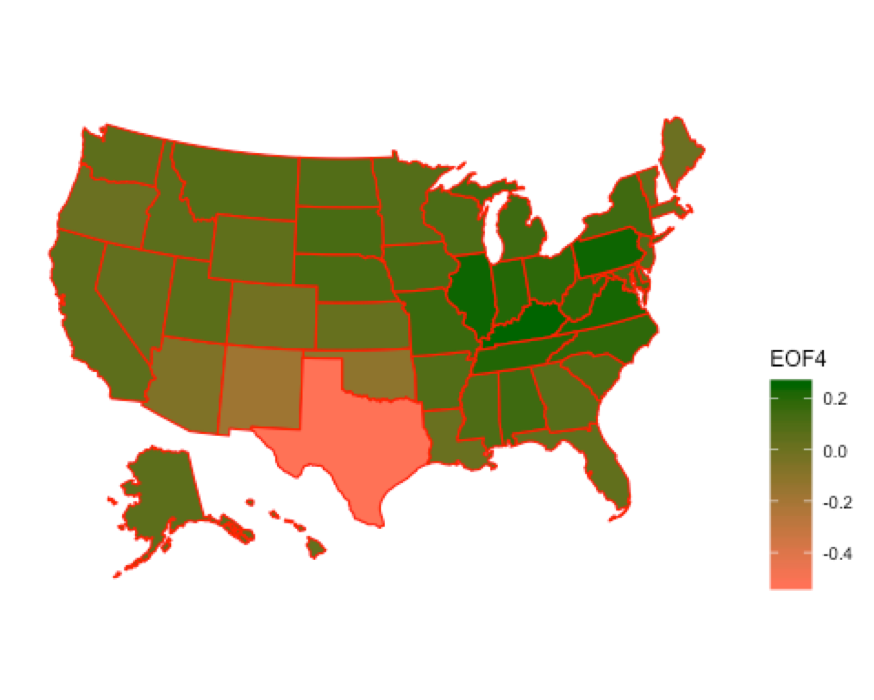
\includegraphics[width=0.70\linewidth]{figures/ch5/SVD/eof4.png}
            \caption{\label{fig:EOF_4} Mask mapping state wise of U4 vector of matrix U}
    \end{figure}
    
    Figure~\ref{fig:EOF_4} notice that the anomaly values are not changing much compare to previous one, more research needs to be done to get more accurate results
    
     \begin{figure}[H]
            \centering
            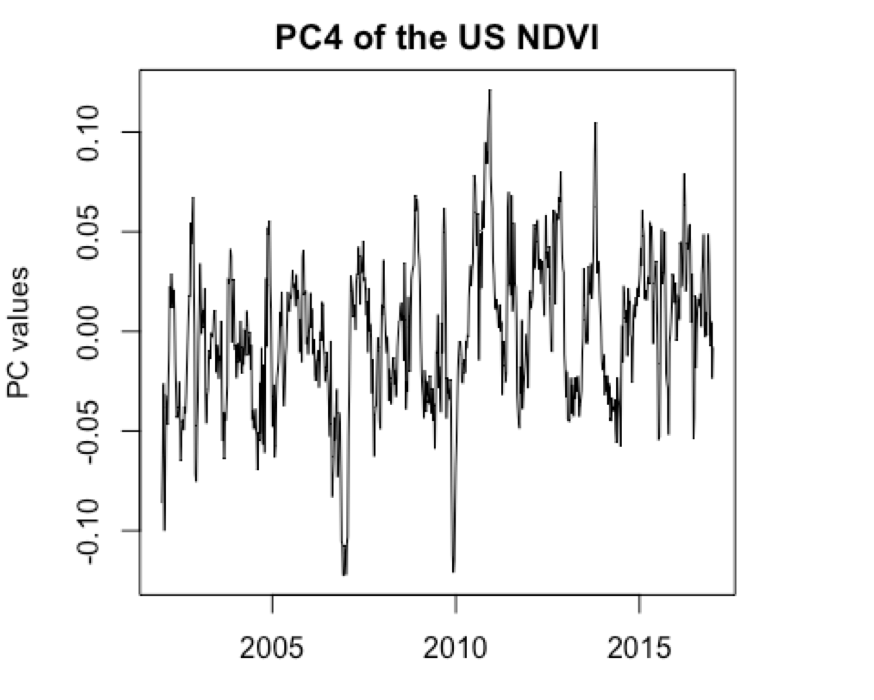
\includegraphics[width=0.70\linewidth]{figures/ch5/SVD/pc4.png}
            \caption{\label{fig:V_4} Time series analysis of V4 vector of matrix V}
    \end{figure}
    
    Figure~\ref{fig:V_4} shows extreme global minimum in 2007 and 2012. Global maximum in 2012. 


     \begin{figure}[H]
            \centering
            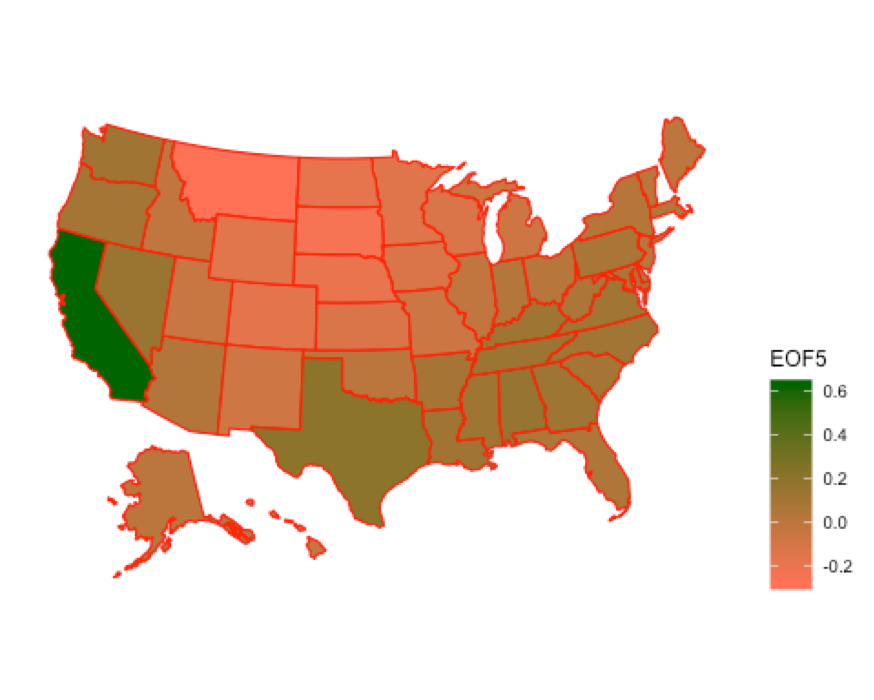
\includegraphics[width=0.70\linewidth]{figures/ch5/SVD/eof5.png}
            \caption{\label{fig:EOF_5} Mask mapping state wise of U5 vector of matrix U}
    \end{figure}
    
    Figure~\ref{fig:EOF_5} shows how anomaly across the united states is evenly spread with the exception of California.
    
     \begin{figure}[H]
            \centering
            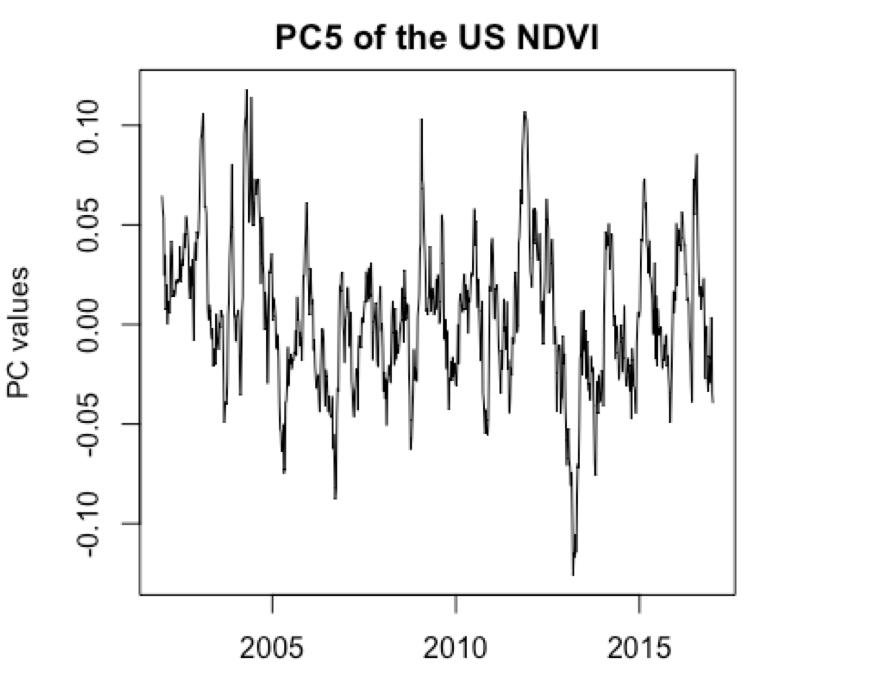
\includegraphics[width=0.70\linewidth]{figures/ch5/SVD/pc5.png}
            \caption{\label{fig:V_5} Time series analysis of V5 vector of matrix V}
    \end{figure}
    
    Figure~\ref{fig:V_5} shows the minimum and maximum values on 2005, 2006, 2007, 2009, and 2012.